% \chapter[误差反馈随机映射卷积神经网络预测模型构造方法]{误差反馈随机映射卷积神经网络预测模型构造方法
% \footnote[11]{本章主要内容已发表在:Zhang, Xinze, Kun He, and Yukun Bao. "Error-feedback stochastic modeling strategy for time series forecasting wi th convolutional neural networks." Neurocomputing 459 (2021): 234-248.}
% }

\chapter{基于卷积结构的SDNN预测模型构造与优化方法 \label{sec:chapter.cnn}
% \footnote[11]{本章主要内容已发表在:Zhang, Xinze, Kun He, and Yukun Bao. "Error-feedback stochastic modeling strategy for time series forecasting wi th convolutional neural networks." Neurocomputing 459 (2021): 234-248.}
}

\section{引言}
% 基于深度学习的时间序列预测建模技术在众多现实决策问题中发挥了重要作用。
% 发明准确高效的时间序列预测建模技术具有重要的理论意义和现实应用价值。
近年来,作为深度神经网络(DNN)的代表结构之一,基于卷积结构的卷积神经网络(CNN)因其优异的特征提取能力与学习能力已被广泛地应用于时间序列预测建模问题中~\cite{sezer2018algorithmic,cavalliCNNbased2021,sadaei2019short}。
然而,如何基于时间序列数据自适应地选择模型结构与参数是应用CNN预测建模技术中的关键挑战。
对于模型选择问题,已有众多研究者展开了相关研究。
Elsken et al.~\cite{elskenNeural2019a}对神经网络模型的既有模型选择方法进行了研究综述,总结出定义神经网络参数搜索空间、针对参数训练模型和基于训练模型结构对所搜索参数加以优化的模型选择范式。
但是,这种传统的模型选择范式需要消耗大量的计算资源与训练时间,使得卷积神经网络时间序列预测建模技术的现实应用面临参数构造难、计算开销大等阻碍~\cite{zela2018towards}。

相较于有训练权重参数的CNN模型,采用随机映射方法构造的CNN模型在图像风格迁移、语音合成、函数拟合等问题中展现出充分潜力~\cite{hePowerful2016,antogniniAudio2019,yuImpact2019}。
这种基于随机映射的CNN模型具有计算开销低、收敛速度快、学习性能好等特点,但也存在网络结构设计难、随机权重输出结果不稳定等问题。
针对时间序列预测问题,Yu et al.~\cite{yuImpact2019}通过将CNN模型中的卷积权重随机初始化并固定,利用最小二乘法闭式求解输出权重,建立了随机卷积神经网络预测模型,并结合合成时间序列数据和煤气供应数据,验证了其方法的可行性。
但此预测建模方法存在若干问题。首先,其卷积结构的选择依赖于人工经验,使得模型无法根据不同预测情景自适应选择合适参数;其次,输出权重全局更新的求解方式,随着卷积核数量的增加,将使卷积层的隐藏特征维度倍数增加,导致求解输出权重的最小二乘法出现病态矩阵问题,削弱了模型的稳定性,甚至使模型出现欠拟合的问题。
因此,如何建立基于卷积结构的随机深度神经网络(SDNN)预测模型的新颖构造及自适应优化方法,解决已有卷积结构SDNN预测建模技术中参数选择时的人工依赖、输出权重求解时的病态矩阵和预测过程的不稳定性,以有效利用随机映射方法的效率优势与卷积结构的学习能力,是本章的研究重点。

为此,本章在已有研究的基础上,针对基于卷积结构的SDNN预测模型构造与自适应优化问题,创新地提出了一种基于误差反馈随机建模(Error-feedback stochastic modeling, ESM)和贪心搜索选择的CNN构造与优化方法(ESM-CNN)。在ESM-CNN这一卷积结构的SDNN预测模型构造与优化方法中,ESM策略通过递归生成随机映射卷积核的方式提高了模型构造效率,并借助误差反馈策略,单独求解各卷积核输出权重,保证了所构造模型的理论收敛性,以此高效构造出具有理论收敛性的预测模型;同时,通过贪心算法解决模型构造中随机映射卷积核的选择问题,使得ESM-CNN能够自适应的在单卷积层内具备不同卷积宽度的卷积核,以此增强了ESM-CNN学习不同尺度时间序列特征的能力,进一步地提高了模型预测性能;最后,采用合成数据和多个真实数据集充分验证了ESM-CNN的有效性以及卷积核选择方法的必要性,与传统随机多层感知机(SMLP)模型和梯度下降训练DNN模型相比,ESM-CNN具有优秀的预测性能与建模效率,是解决时间序列预测问题的有效方法。



本章的主要内容包括:\secref{sec:esm.cnn}简要介绍了传统CNN预测模型的构造过程,并对本章节所提出的ESM-CNN模型构造与优化方法进行了详细阐述;\secref{sec:esm.exp}从数据集选取、对比模型选取、评价指标选取、实验流程和实验环境等方面介绍了本章的实验方案;\secref{sec:esm.ana}比较、分析和总结了各模型在所选数据集上的实验结果;最后,\secref{sec:esm.conc}对本章予以小结。

\section{ESM-CNN预测模型 \label{sec:esm.cnn}}

\subsection{CNN预测模型}
卷积神经网络(CNN)是将输入连接卷积核做局部非线性变换,并池化展开特征图所构成的神经网络~\cite{lecun1995convolutional}。
卷积是指输入的滑动局部非线性变换。
通过对时间序列输入特征的卷积操作,卷积核(Convolutional filter)能够基于完整输入学习出有用的非线性特征,并建立起所学习特征与对应卷积核宽度(Filter size)输入的关系,由此组成了卷积层(Convolutional layer)的输出特征图(Feature map)。这些特征图往往被送入池化层(Pooling layer)进行下采样(Subsample)以降低卷积层的输出带宽(Output band),同时增强神经网络对异常特征图值的鲁棒性~\cite{yang2015deep,zhao2017convolutional,koprinskaConvolutional2018}。
池化操作后的特征图会继续送入神经网络的下一层结构中,以学习更抽象的表示或生成输出结果。

这里,本节对一种典型结构CNN预测模型进行具体介绍,该模型由生成特征图的单卷积层、进行下采样的平均池化层(Pooling layer)和生成预测结果的全连接层(Fully connected layer)组成。
对于由$N$个样本组成的时间序列数据$D=\left\{\left(X_{i}, Y_{i}\right) \in\left(\mathbb{R}^{T} \times \mathbb{R}^{H}\right)\right\}_{i=1}^{N}$,其中$X_i$表示历史T步内的时间序列观测值$X_i = [x_1,\dots, x_T]^{\trans}$,$Y_i$表示预测时长H步内的时间序列观测值$Y_i = [x_{T+1},\dots, x_{T+H}]^{\trans}$。一个具有$C$个卷积核的CNN预测模型可表示为如\autoref{eq:conv},\autoref{eq:pool}和\autoref{eq:sec.cnn.fc}所示过程:
\begin{align}
    m_j^t &= \sigma \left(\sum^{K_m}_{k_m=1} w^{k_m}_j x_{t+k_m-1} +b_j\right), \quad &t &= 1,\dots, T-K_m +1, \label{eq:conv}  \\
    p_j^i &= \frac{\sum^{K_p}_{k_p=1} m_j^{i+k_p-1}}{K_p}, \quad &i &= 1,..., T-K_p - K_m+2, \label{eq:pool} \\
    f_C &= \sum^C_{j=1} \left( \sum^{T-K+2}_{i=1}\beta_{j}^i p_j^i\right) + \beta_0.& & \label{eq:sec.cnn.fc}
\end{align}

\autoref{eq:sec.cnn.fc}中,$K = K_p + K_m$,$K_p$和$K_m$分别为池化操作与卷积操作的宽度大小。
\autoref{eq:pool}中,${m}_j$为特征图向量$[m_j^1, \ldots, m^{T-{K_m}+1}_j]^{\mathrm{T}}$,基于第$j$个卷积在输入时间序列做如\autoref{eq:conv}所示的卷积操作后得到。
$\sigma(\cdot)$表示卷积核所使用的激活函数。在本章节中,$\sigma(\cdot)$为sigmoid激活函数。
${w_j} = [w_j^1,\ldots, w_j^{K_m}]$和$b_j$分别为第$j$个卷积核的权重与偏置项。
$p_j$表示对${m}_j$做如\autoref{eq:pool}所示平均池化操作后的池化特征图向量$[p_j^1, \ldots, p^{T-{K}+2}_j]^{\mathrm{T}}$。
$[\beta_1^1, \beta_1^2,\ldots,\beta_C^{T-K+2}]$和$\beta_0$为第$j$个卷积核与输出层间的全连接层权重与偏置项,$\beta_j^i = [\beta_{j}^{i,1},\ldots,\beta_{j}^{i,H}]^{\mathrm{T}}$。

\begin{figure*}[!t]
    \centering
    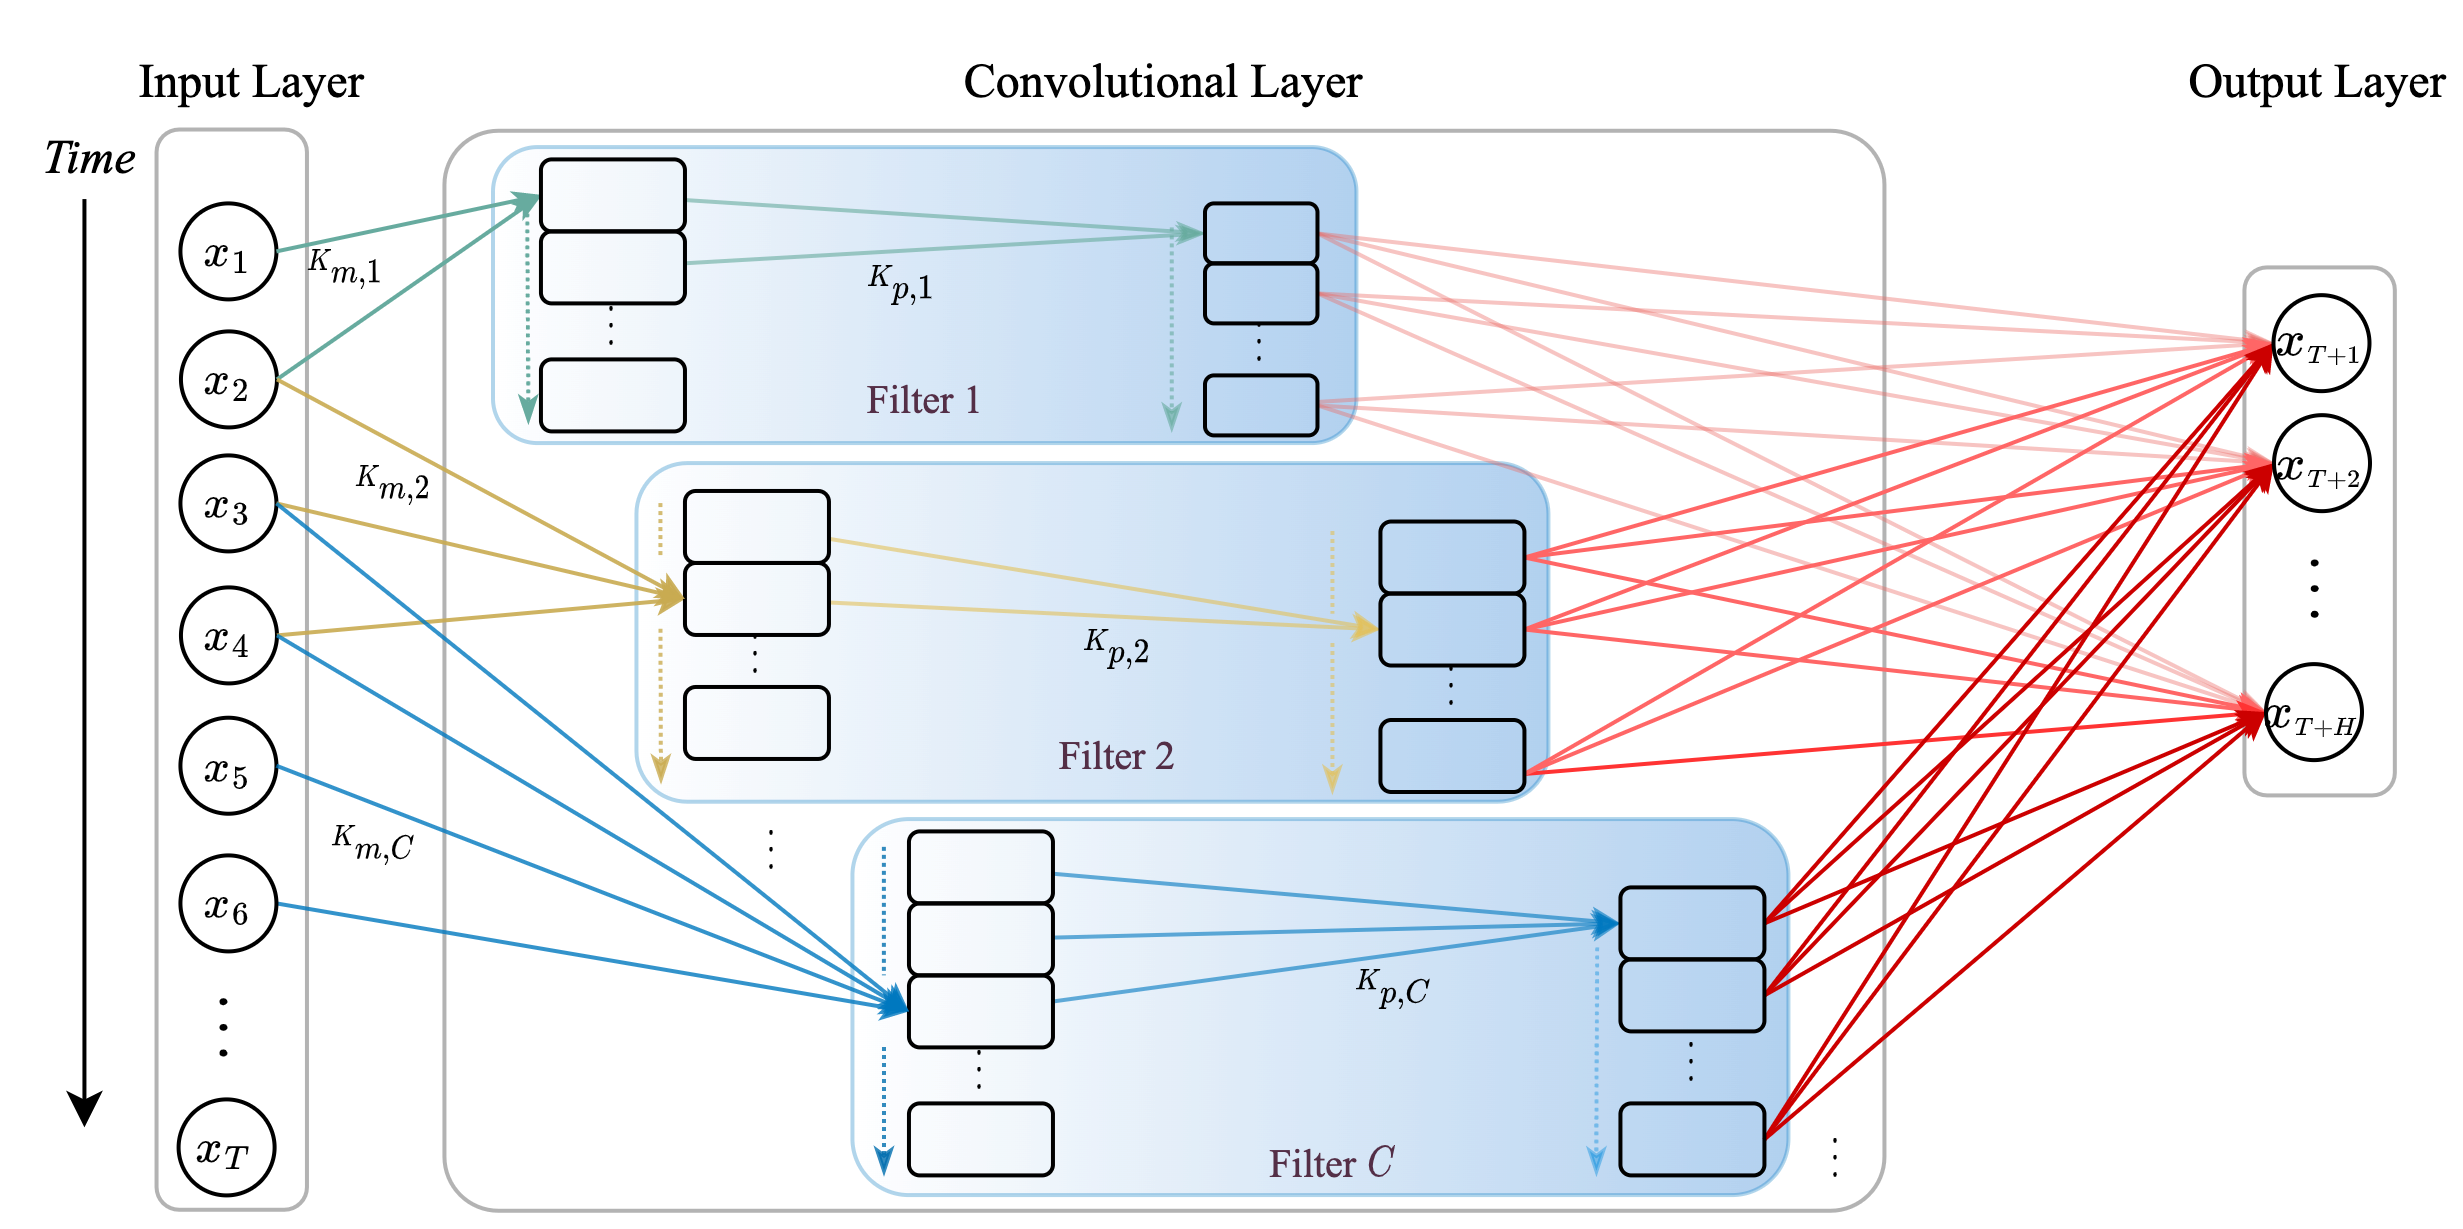
\includegraphics[width = \textwidth]{float/ch.cnn/esm-cnn.png}
    \caption{\label{fig:esm_arch} ESM-CNN预测模型神经网络结构}
\end{figure*}

在传统的CNN预测模型构造方法中,通过以减小预测误差$\| e \|$为目标,梯度下降训练包含所有权重项与偏置项在内的权重参数,CNN能够有效学习出历史输入时间序列与预测目标时间序列间的函数关系,生成良好的预测结果。
但这种构造方法需要预先定义包含卷积核宽度、卷积核数量、梯度下降学习速率等众多超参数(Hyper-parameters),进过反复迭代训练评价后,才能选择出合适的超参与权重参数组合。此过程往往会消耗大量的计算资源和时间,存在显著的改进空间。


为解决现有CNN预测建模技术模型选择困难、计算开销高等问题,本章提出了一种误差反馈随机建模(ESM)构造策略,结合基于贪心算法的卷积核选择算法,建立ESM-CNN预测模型。该模型神经网络结构如\autoref{fig:esm_arch}所示,其中绿色线、黄色线和蓝色线分别表示不同结构随机卷积核的卷积与池化操作,深浅不同的红色线表示迭代局部更新的输出权重,同一深度的红色线表示链接同一卷积核的输出权重。

\subsection{误差反馈随机建模策略\label{sec:esm.esm}}
为高效构造具备可靠预测性能的卷积结构SDNN预测模型,利用随机映射方法的优异建模效率,同时解决随机映射算法对预测性能稳定性的干扰,本节提出了一种ESM策略,建立CNN构型下的SDNN预测模型。
该方法通过在单卷积层内递归增长添加固定随机初始化权重卷积核的方式构造CNN隐藏结构,同时利用误差反馈闭式计算新增卷积核所对应的输出权重参数,以此完成整个预测模型的构造过程,同时为模型的预测函数拟合能力提供理论收敛保证。

具体地,对于一个已具有$C$个卷积核的单卷积层ESM-CNN,其模型可被公式表述为:
\begin{equation}
    \label{eq:sccnn}
    f_C = \sum^C_{j=1} \left( \sum^{T-K+2}_{i=1}\beta_{j}^i p_j^i + \beta^0_j \right),
\end{equation}
并进一步简写为:$f_C= \sum^C_{j=1}\sum^{T-K+2}_{i=0} \beta_j^i p_j^i$。



\autoref{eq:sccnn}中,$\beta_j = [\beta_j^0, \beta_j^1, \ldots, \beta_j^{T-K+2}]$ 表示全连接输出层中连接第$j$个卷积核池化特征图向量与输出单元的权重参数,$p_j^0 = I$。
ESM-CNN的预测误差如\autoref{eq:sec.cnn.error}所示:
\begin{equation}
    e_C = Y- f_C = [e_C^1,\ldots, e_C^H]. \label{eq:sec.cnn.error}
\end{equation}

若预测模型的均方误差(Mean square error,MSE)未降低至容忍水平$\varrho$,ESM策略将继续新增一个随机映射卷积核$m_{C+1}$生成对应的池化特征图向量$p_{C+1}$,并将$p_{C+1}$全连接至输出层中以加宽模型隐藏结构。
其中,新增卷积核所对应的全连接输出层权重将基于当前模型的预测误差$e_C$反馈,通过如\autoref{eq:scupdate}最小二乘法加以求解:
\begin{equation}\label{eq:scupdate}
    \left[\beta_{{C+1}}^0, \ldots, \beta_{{C+1}}^{T-K+2} \right]=\argmin _{\beta}\|e_C -\sum_{i=0}^{T-K+2} \beta_{C+1}^i p_{C+1}^i \|.
\end{equation}

通过此策略,所构造的ESM-CNN预测模型能够具备随着卷积核数量增加而单调下降并收敛的预测误差,从而完成对预测目标函数的逼近。该性质通过如下代数推导予以证明:
\begin{proof}

    定义ESM-CNN的预测误差中间项为:$\tilde{e}_{C+1}^{\, 0}, \ldots, \tilde{e}_{C+1}^{\, T-K+2} $,新增卷积核所对应的全连接输出层权重中间项为:$\tilde{\beta}_{C+1}^{\, 0}, \ldots, \tilde{\beta}_{C+1}^{\, T-K+2}$,中间项之间的计算关系为:
    \begin{alignat*}{2}
        & \tilde{e}_{C+1}^{\, i+1}       & = & \mspace{18mu} \tilde{e}_{C+1}^{\, i}-\tilde{\beta}_{C+1}^{\, i+1} p_{C+1}^{i+1}, \quad i = 0,\ldots,T-K+1,                                        \\
       \shortintertext{其中,}
        & \tilde{\beta}_{C+1}^{\, i+1}   & = & \mspace{18mu} [\tilde{\beta}_{C+1}^{\, i+1,1}, \ldots,\tilde{\beta}_{C+1}^{\, i+1,h},\ldots, \tilde{\beta}_{C+1}^{\, i+1,H}],                     \\
        & \tilde{\beta}_{C+1}^{\, i+1,h} & = & \mspace{18mu} \left\langle \tilde{e}_{C+1}^{\, i,h}, p_{C+1}^{\, i+1}\right\rangle /\left\|p_{C+1}^{\, i+1}\right\|^{2} , \quad h= 1, \ldots, H , \\
       \shortintertext{同时,}
        & \tilde{e}_{C+1}^{\, 0}         & = & \mspace{18mu} e_{C}- \tilde{\beta}_{C+1}^{\, 0} p_{C+1}^{\, 0},                                                                                   \\
        & \tilde{\beta}_{C+1}^{\, 0}   & = & \mspace{18mu} [\tilde{\beta}_{C+1}^{\, 0,1}, \ldots,\tilde{\beta}_{C+1}^{\, 0,h},\ldots, \tilde{\beta}_{C+1}^{\, 0,H}],                     \\
        & \tilde{\beta}_{C+1}^{\, 0,h} & = & \mspace{18mu} \left\langle {e}_{C}^{\, h}, p_{C+1}^{\, 0}\right\rangle /\left\|p_{C+1}^{\, 0}\right\|^{2} , \quad h= 1, \ldots, H , \\
        % \shortintertext{可得:}
        & \tilde{e}_{C+1}^{\, T-K+2} \,  & = & \mspace{18mu} {e}_{C} - \sum^{T-K+2}_{i=0} \tilde{\beta}_{C+1}^{\, i} p_{C+1}^{\, i}.
   \end{alignat*}
因新增卷积核所对应的全连接输出层权重基于最小二乘法予以求解:
$$
\left[\beta_{{C+1}}^0, \ldots, \beta_{{C+1}}^{T-K+2} \right]=\argmin _{\beta} \,\|e_C -\sum_{i=0}^{T-K+2} \beta_{C+1}^i p_{C+1}^i \|,
$$
则$\left\|e_{C+1}\right\|^{2}$与$\left\|\tilde{e}_{C+1}^{\, T-K+2}\right\|^{2}$存有不等式关系:
$$
    \|e_{C+1}\|^{2} \,= \min _{\beta} \,\| e_C -\sum_{i=0}^{T-K+2} {\beta}_{{C+1}}^i p_{C+1}^i \|^{2}  \, \leq  \| {e}_{C} - \sum^{T-K+2}_{i=0} \tilde{\beta}_{C+1}^{\, i} p_{C+1}^{\, i} \|^{2} \, =  \|\tilde{e}_{C+1}^{\, T-K+2}\|^{2}.
$$
同时,预测误差中间项之前存在着单调下降性质:
\begin{align*}
    & \|\tilde{e}_{C+1}^{\, i+1}\|^2-\|\tilde{e}_{C+1}^{\, i}\|^2 \\
    ={}    & \sum_{h=1}^{H}
    \left(
    \langle \tilde{e}_{C+1}^{\, i,h}-\tilde{\beta}_{C+1}^{\, i+1,h} p_{C+1}^{i+1}
    ,
    \tilde{e}_{C+1}^{\, i,h}-\tilde{\beta}_{C+1}^{\, i+1,h} p_{C+1}^{i+1} \rangle
    -
    \langle \tilde{e}_{C+1}^{\, i,h}, \tilde{e}_{C+1}^{\, i,h} \rangle
    \right)                                                              \\
    ={}    & \sum_{h=1}^{H}
    \left(
    \langle \tilde{\beta}_{C+1}^{\, i+1} p_{C+1}^{i+1}
    ,
    \tilde{\beta}_{C+1}^{\, i+1} p_{C+1}^{i+1} \rangle
    -
    2 \langle \tilde{e}_{C+1}^{\, i,h} , \tilde{\beta}_{C+1}^{\, i+1} p_{C+1}^{i+1} \rangle
    \right)                                                              
    \\
    ={}    & \sum_{h=1}^{H}
    \left(
    \langle 
    \frac{\left\langle \tilde{e}_{C+1}^{\, i,h}, p_{C+1}^{\, i+1}\right\rangle}{\left\|p_{C+1}^{\, i+1}\right\|^{2}}  
    p_{C+1}^{i+1}
    ,
    \frac{\left\langle \tilde{e}_{C+1}^{\, i,h}, p_{C+1}^{\, i+1}\right\rangle}{\left\|p_{C+1}^{\, i+1}\right\|^{2}}  
    p_{C+1}^{i+1}
    \rangle
    -
    2 
    \langle 
    \tilde{e}_{C+1}^{\, i,h} 
    ,
    \frac{\left\langle \tilde{e}_{C+1}^{\, i,h}, p_{C+1}^{\, i+1}\right\rangle}{\left\|p_{C+1}^{\, i+1}\right\|^{2}}  
    p_{C+1}^{i+1} 
    \rangle
    \right)                                                              
    \\
    ={}    & \sum_{h=1}^{H}
    \left(
    \frac{{\left\langle \tilde{e}_{C+1}^{\, i,h}, p_{C+1}^{\, i+1}\right\rangle}^2}{\left\|p_{C+1}^{\, i+1}\right\|^{4}}  
    \langle 
    p_{C+1}^{i+1}
    ,
    p_{C+1}^{i+1}
    \rangle
    -
    2 \frac{\left\langle \tilde{e}_{C+1}^{\, i,h}, p_{C+1}^{\, i+1}\right\rangle}{\left\|p_{C+1}^{\, i+1}\right\|^{2}}  
    \langle \tilde{e}_{C+1}^{\, i,h} 
    ,
    p_{C+1}^{i+1} 
    \rangle
    \right)                                                              
    \\
    ={}    & \sum_{h=1}^{H}
    \left(
    \frac{{\left\langle \tilde{e}_{C+1}^{\, i,h}, p_{C+1}^{\, i+1}\right\rangle}^2}{\left\|p_{C+1}^{\, i+1}\right\|^{4}}  
    {\left\|p_{C+1}^{\, i+1}\right\|^{2}}  
    -
    2 \frac{{\left\langle \tilde{e}_{C+1}^{\, i,h}, p_{C+1}^{\, i+1}\right\rangle}^2}{\left\|p_{C+1}^{\, i+1}\right\|^{2}}  
    \right)                                                              
    \\        
    ={}    & \sum_{h=1}^{H}
    \left(
    - {\langle \tilde{e}_{C+1}^{\, i,h}, p_{C+1}^{\, i+1} \rangle}^2 / \left\|p_{C+1}^{\, i+1}\right\|^{2}
    \right)                                                              \\
    \leq{} & 0 .
    \end{align*}
该性质在$\left\|\tilde{e}_{C+1}^{\, 0}\right\|^{2}$与$\left\|e_{C}\right\|^{2}$间仍然保持:
\begin{align*}
    & \|\tilde{e}_{C+1}^{\,0}\|^2-\|{e}_{C}\|^2 \\
    ={}    & \sum_{h=1}^{H}
    \left(
    \langle {e}_{C}^{\, h}-\tilde{\beta}_{C+1}^{\, 0,h} p_{C+1}^{0}
    ,
    {e}_{C}^{\, h}-\tilde{\beta}_{C+1}^{\, 0,h} p_{C+1}^{0} \rangle
    -
    \langle {e}_{C}^{\, h}, {e}_{C}^{\, h} \rangle
    \right)                                                              \\
    ={}    & \sum_{h=1}^{H}
    \left(
    \langle \tilde{\beta}_{C+1}^{\, 0,h} p_{C+1}^{0}
    ,
    \tilde{\beta}_{C+1}^{\, 0,h} p_{C+1}^{0} \rangle
    -
    2 \langle {e}_{C}^{\, h} , \tilde{\beta}_{C+1}^{\, 0,h} p_{C+1}^{0} \rangle
    \right)                                                              
    \\
    ={}    & \sum_{h=1}^{H}
    \left(
    \langle 
    \frac{\left\langle {e}_{C}^{\, h}, p_{C+1}^{\, 0}\right\rangle}{\left\|p_{C+1}^{\, 0}\right\|^{2}}  
    p_{C+1}^{0}
    ,
    \frac{\left\langle {e}_{C}^{\, h}, p_{C+1}^{\, 0}\right\rangle}{\left\|p_{C+1}^{\, 0}\right\|^{2}}  
    p_{C+1}^{0}
    \rangle
    -
    2 
    \langle 
    {e}_{C}^{\, h} 
    ,
    \frac{\left\langle {e}_{C}^{\, h}, p_{C+1}^{\, 0}\right\rangle}{\left\|p_{C+1}^{\, 0}\right\|^{2}}  
    p_{C+1}^{0} 
    \rangle
    \right)                                                              
    \\
    ={}    & \sum_{h=1}^{H}
    \left(
    \frac{{\left\langle {e}_{C}^{\, h}, p_{C+1}^{\, 0}\right\rangle}^2}{\left\|p_{C+1}^{\, 0}\right\|^{4}}  
    \langle 
    p_{C+1}^{0}
    ,
    p_{C+1}^{0}
    \rangle
    -
    2 \frac{\left\langle {e}_{C}^{\, h}, p_{C+1}^{\, 0}\right\rangle}{\left\|p_{C+1}^{\, 0}\right\|^{2}}  
    \langle {e}_{C}^{\, h} 
    ,
    p_{C+1}^{0} 
    \rangle
    \right)                                                              
    \\
    ={}    & \sum_{h=1}^{H}
    \left(
    \frac{{\left\langle {e}_{C}^{\, h}, p_{C+1}^{\, 0}\right\rangle}^2}{\left\|p_{C+1}^{\, 0}\right\|^{4}}  
    {\left\|p_{C+1}^{\, 0}\right\|^{2}}  
    -
    2 \frac{{\left\langle {e}_{C}^{\, h}, p_{C+1}^{\, 0}\right\rangle}^2}{\left\|p_{C+1}^{\, 0}\right\|^{2}}  
    \right)                                                              
    \\        
    ={}    & \sum_{h=1}^{H}
    \left(
    - {\langle {e}_{C}^{\, h}, p_{C+1}^{\, 0} \rangle}^2 / \left\|p_{C+1}^{\, 0}\right\|^{2}
    \right)                                                              \\
    \leq{} & 0 .
    \end{align*}
因此,ESM-CNN的预测误差收敛性可证:
$$
\|e_{C+1}\|^2  \; \leq \|\tilde{e}_{C+1}^{\, T-K+2}\|^2 \; \leq \|\tilde{e}_{C+1}^{\,0}\|^2 \; \leq \|{e}_{C}\|^2 .
$$
\NoEndMark
\end{proof}

与全局更新输出层权重的构造方式不同,本章所提出的ESM构造策略通过误差反馈迭代局部更新输出层权重的方式完成输出层权重的计算。具体地,ESM构造策略具备以下三种优势:1)与全局更新输出层权重相比,迭代局部更新输出层权重的方式具有更小的计算开销,这种低开销优势会随隐藏层结构的增大同时扩大;2)随着卷积层中递归新增卷积核的不断加入,链接至输出层的池化特征图向量维度会同时倍数增大,与预测目标维度相比过大的特征维度会导致闭式求解算法的病态问题(Ill-posed problem)\cite{vogel2002computational},进而破坏预测性能的稳定性和鲁棒性;3)基于误差反馈递归更新输出权重构造的预测模型能在神经网络隐藏构造的过程中不断弥补上步预测误差,同时,这种历史输出权重保持固定的方式在一定程度上承担了正则化的作用,从而增强了所构造模型的性能稳定性。

\subsection{卷积参数贪心选择方法
\label{sec:chapCNN.greedy}}
针对ESM-CNN预测模型构造过程中的卷积核选择问题,本章节提出了一种基于贪心算法的卷积核选择方法,使得ESM-CNN具有在单卷积层中同时具备不同宽度的卷积核结构,以此增强模型对于不同尺度时间序列特征的学习建模能力。

对于如\autoref{eq:sccnn}所示具有$C$个卷积核的单卷积层ESM-CNN,在新增卷积核结构时,基于均匀分布(Uniform distribution)$[-\lambda, \lambda]$、卷积与池化宽度$\{(K_{m,s}, K_{p,s})\}^S_{s=1}$生成一批对应的池化特征图向量 $\{p_{{C+1},s} \}^S_{s=1}$表示对应的备选卷积核结构。
为评价这些备选卷积核结构,利用将备选卷积核加入当前网络中所能下降的预测误差,本节提出了一种卷积核评分$\Delta_{{C+1, s}}$,其计算方式如\autoref{eq:filterScore}所示:
\begin{align}
    \Delta_{{C+1},s} & = \| e_{C+1,s} \|^2 - \| e_{C} \|^2 \label{eq:filterScore}                                                                      \\
    {}               & = \|\ e_C -\sum_{i=0}^{T-K^{\prime}+2} \beta_{C+1, s}^i p_{C+1, s}^i \|^2 -  \| e_{C} \|^2, \notag  
\end{align}

\autoref{eq:filterScore}中,$K^{\prime} = K_{m,s} + K_{p,s}$,$p^i_{C+1, s}$和$\beta^i_{C+1, s}$分别由\autoref{eq:pool}和\autoref{eq:scupdate}计算得出。
基于所提出的卷积核评分$\Delta_{{C+1, s}}$,将实现最好预测效果提升的备选卷积核$p_{C+1}^{*}$选出,作为新增卷积核正式加入当前神经网络结构,该过程如\autoref{eq:scselection}所示:
\begin{equation}\label{eq:scselection}
    p_{C+1}^{*} = \argmax\limits_{p_{{C+1},s}} \{ \Delta_{{C+1},s}, s = 1,\ldots,S \}.
\end{equation}

在此之后,新增卷积核所对应的全连接输出层权重通过\ref{eq:scupdate}求解得出。结合本章节所提出的ESM构造策略与卷积核选择方法,高效构造出一种具备多尺度时间序列特征学习能力、预测函数拟合收敛性和稳定预测性能的ESM-CNN预测模型。
% \autoref{fig:esm_arch}详细描绘了ESM-CMM预测模型的神经网络结构。

\begin{figure*}[!t]
    \centering
    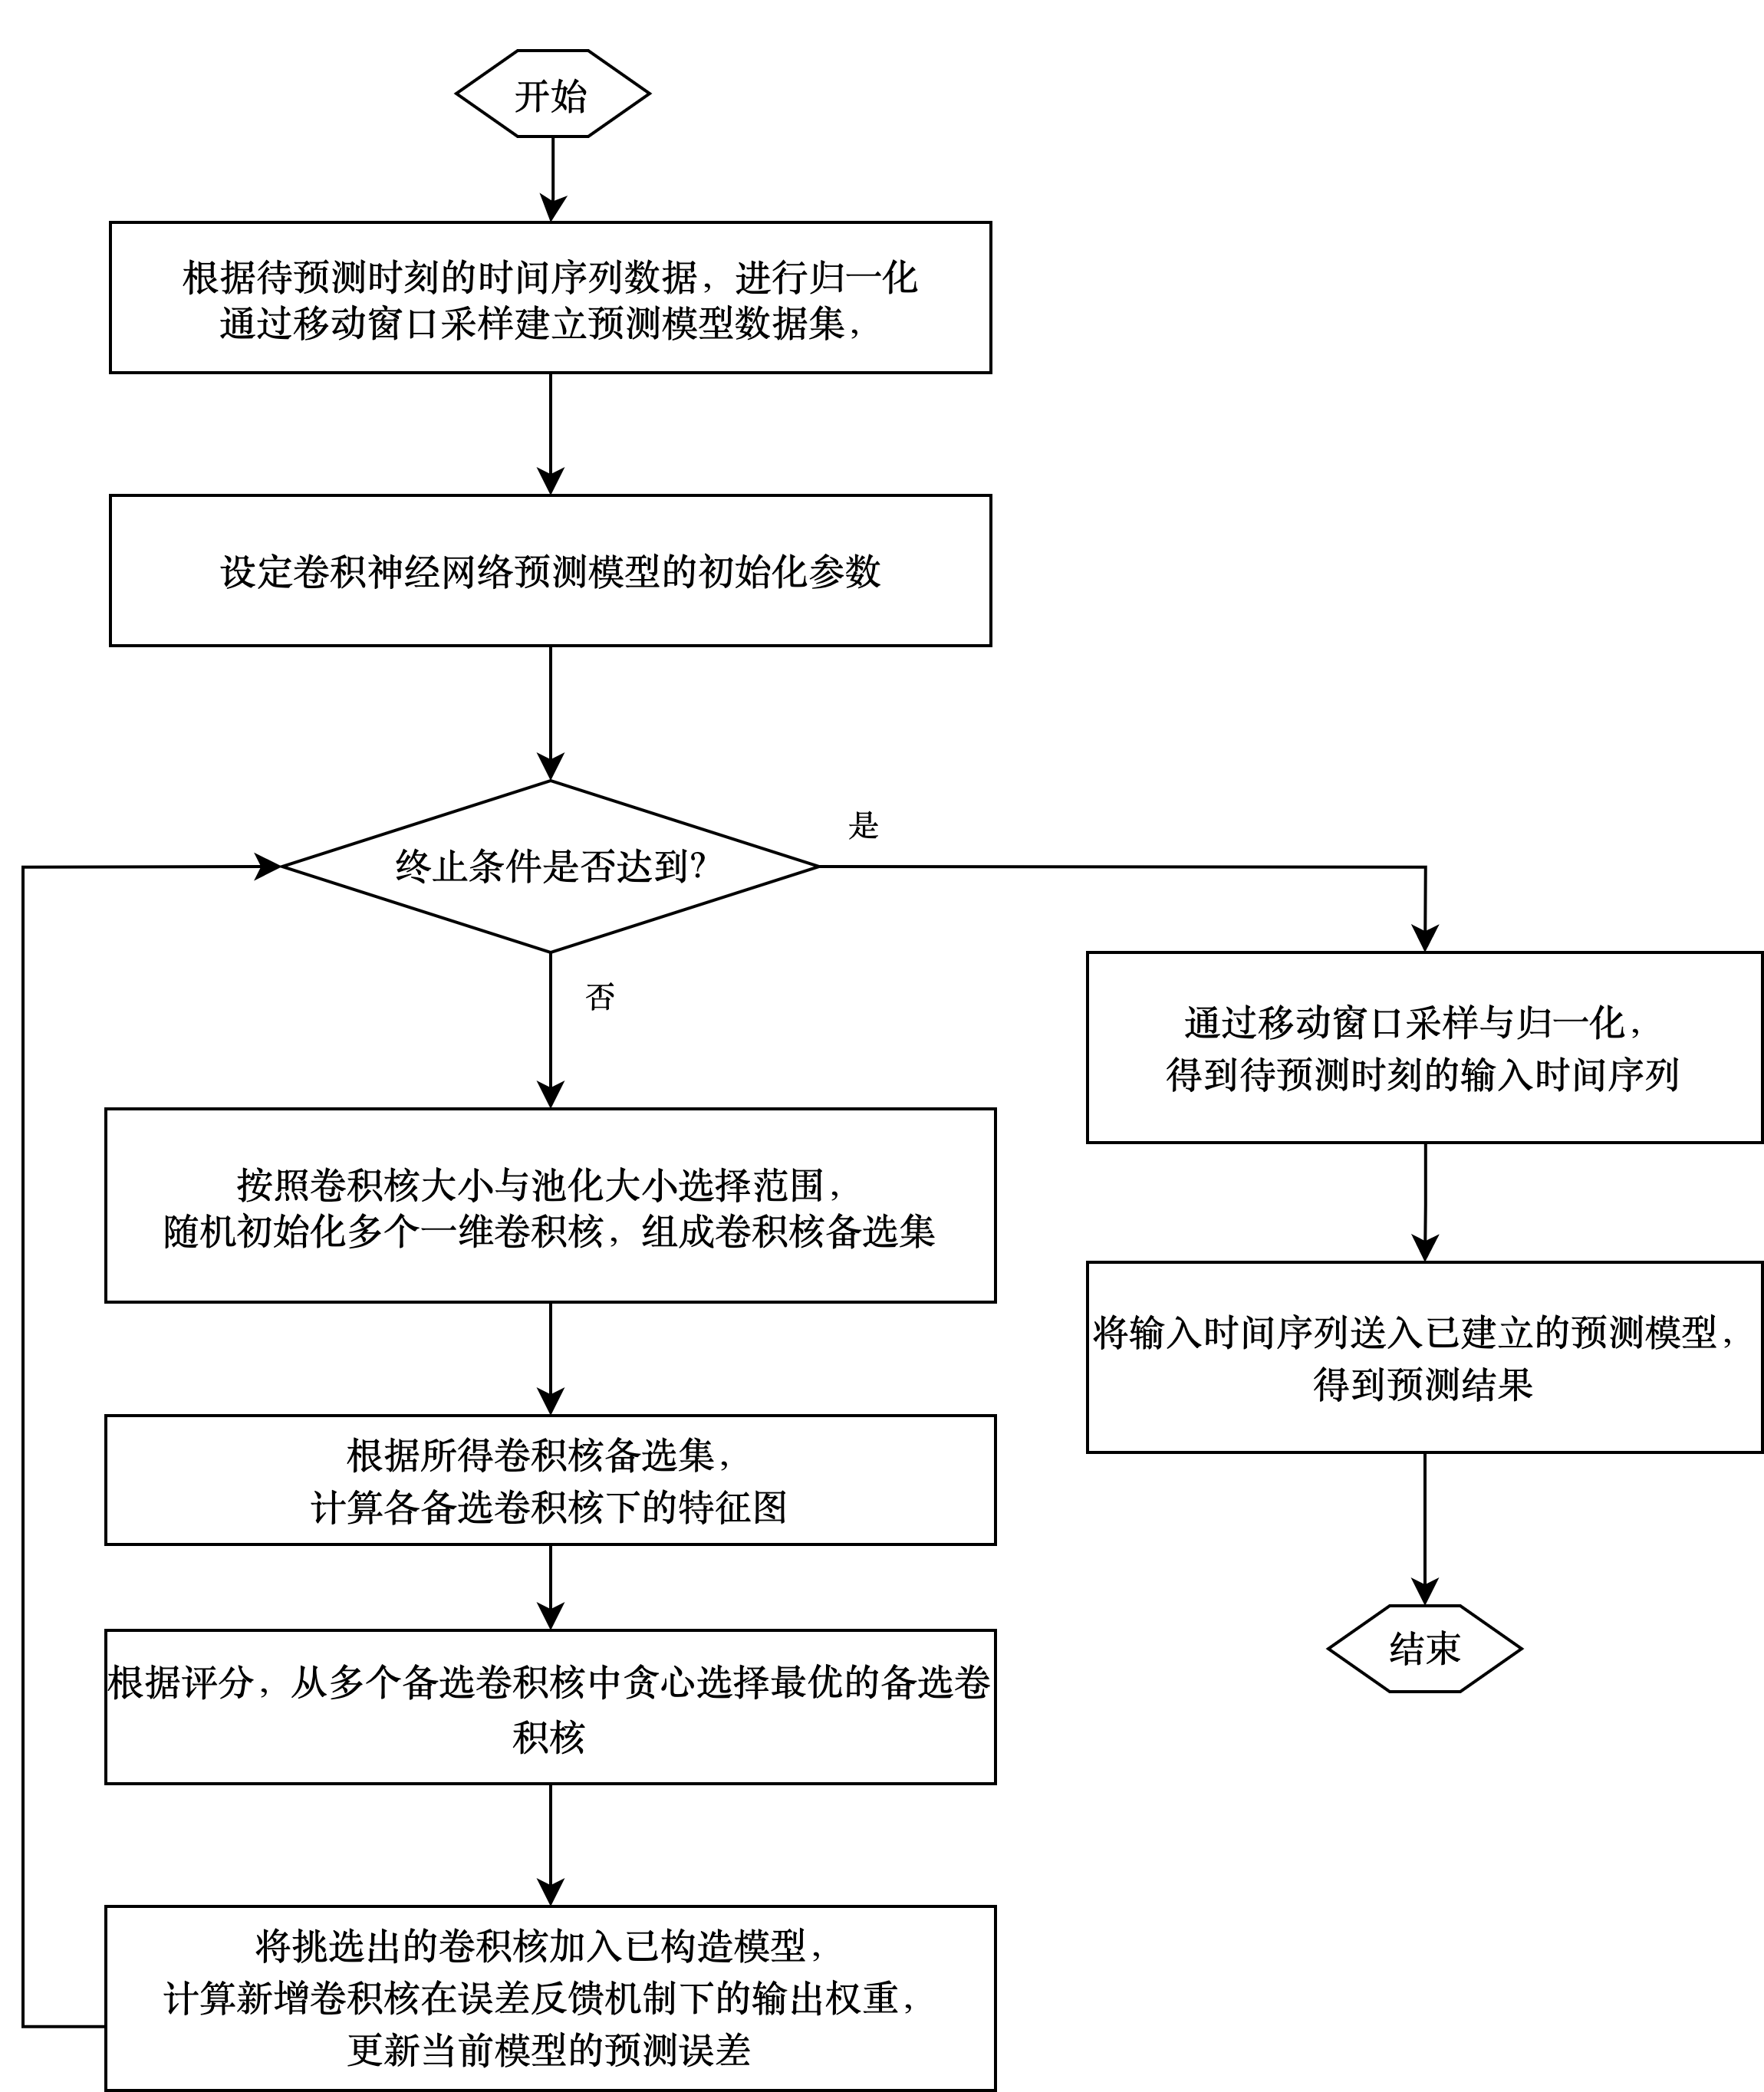
\includegraphics[width = 0.8\textwidth]{float/ch.cnn/flow.png}
    \caption{\label{fig:flowchart} ESM-CNN预测模型构造过程}
\end{figure*}

\subsection{ESM-CNN构造过程}
如\autoref{fig:flowchart}所示,ESM-CNN预测模型的构造过程主要包含:预处理、初始化、评价和更新四个环节。
具体地,所述模型及构造过程为:

(1)对于时间序列数据,构造训练数据集$D=\left\{\left(X_{i}, Y_{i}\right) \in\left(\mathbb{R}^{T} \times \mathbb{R}^{H}\right)\right\}_{i=1}^{N}$,并将数据集$D$归一化至标准正态分布。其中,$N$为数据集$D$中的总样本数,数据集中样本$(X_i,Y_i )$由包含历史T时刻内的时间序列数据$[x_1,\ldots,x_T ]^{\trans}$和未来H步时刻内的时间序列预测目标$[x_{T+1},\ldots,x_{T+H}]^{\trans}$组成。

(2) 设定ESM-CNN预测模型的初始化参数,包括容忍水平$\varrho $,最大特征图通道数$C_{\max}$,初始预测误差$e_0 = [x_{T+1},\ldots,x_{T+H}]^{\trans}$,卷积核宽度$K_m$选择范围$M=\{ K_{m,s}\}^S_{s=1}$与池化操作宽度挑选范围$P=\{K_{p,s}\}^S_{s=1}$,以及卷积核权重的随机初始化分布$[-\lambda,\lambda]$。

(3)在终止条件为特征图通道数$C\leq C_{\max}$或当前模型预测结果的MSE小于$\varrho $的构造过程中,基于卷积核宽度选择范围$M$与池化操作宽度选择范围$P$,依次从参数组合$(K_{m,s}, K_{p,s})$和均匀分布$[-\lambda,\lambda]$中生成$S$个备选卷积核,以此构成卷积核备选集,并根据得到的备选集,计算各备选卷积核下的池化特征图向量$\{ p_{C+1,s}\}^S_{s=1}$。

(4)基于\autoref{eq:filterScore}计算各备选卷积核的评分,从中贪心选出最优的卷积核结构及对应卷积核权重,将其加入当前神经网络结构中,更新卷积层卷积核数量和模型预测误差。迭代此过程,直至满足终止条件。


\section{实验设计与流程\label{sec:esm.exp}}
\subsection{数据集描述}
为充分评估所提ESM-CNN预测模型的预测性能和验证其收敛能力,本章节在经典人工合成时间序列数据集和多项真实时间序列数据集上进行实验验证研究。实验数据集名称及简写如\autoref{tab:cnn.dataName}所示。
\autoref{tab:app_data}展示了本章节所用数据集的统计信息。其中,第一列、第五列和第六列说明了所用数据集的名称,起始截止日期和大小。
第二列展示所用数据集的平稳性(Stationarity)状态,“\cmark”表示该数据集为平稳的,“\xmark'表示该数据集为非平稳的,该状态通过扩张的迪基-福勒检验(Augmented Dickey Fuller,ADF)\footnote{https://www.statsmodels.org/stable/generated/statsmodels.tsa.stattools.adfuller.html}判断得出。第三列与第四列则分别表示了数据集的趋势性(Trend)与季节性(Seasonality)强度分数\footnote{https://otexts.com/fpp2/seasonal-strength.html},分数越高表明该数据具备越强的趋势性或季节性。各数据集的说明如下:

\begin{table}[!t]
    \centering
    \caption{实验数据集名称及英文缩写对照 \label{tab:cnn.dataName}}
    \begin{tabularx}{\textwidth}{lXl}
        \toprule
        {数据集中文名称} & {数据集英文名称} & 英文缩写 \\  \midrule
        一阶自回归 & First order autoregression & AR1 \\
        比特币两小时美元价格  & Two-hourly bitcoin to U.S. dollar price & BTC          \\
        流感阳性样本率     & Influenza-like illness rate                & ILI          \\
        欧洲布伦特原油周价格  & Weekly Europe Brent crude oil price     & BRENT-weekly \\
        欧洲布伦特原油周价格  & Daily Europe Brent crude oil price      & BRENT-daily  \\
        美国WTI原油周间价格 & Weekly WTI crude oil price              & WTI-weekly   \\
        标普500每日收盘指数 & Daily close value of S\&P 500 index     & S\&P 500     \\
        纳斯达克每日收盘指数  & Daily close value of NASDAQ Composite   & NASDAQ       \\
        道琼斯每日收盘指数   & Daily close value of Dow Jones Average  & DJI          \\
        纽约证交所每日收盘指数 & Daily close value of NYSE Composite     & NYSE         \\
        \bottomrule
        
    \end{tabularx}

\end{table}


\begin{table}[!t]
    \centering
    \caption{数据集信息 \label{tab:app_data}}
    \begin{tabularx}{\textwidth}{lccccY}
    % \caption{数据集信息 \label{tab:app_data}}\\
    \toprule
    数据集名称      & 平稳性 & 趋势性 & 季节性 &  起始截止日期  & 数据集大小 \\ \midrule
    AR1          & \xmark      & 0.97      & 0.09        & -                           & 500         \\
    BTC          & \xmark      & 0.99      & 0.66        & 05/25/2020 $\sim$ 03/20/2021 & 2181        \\
    ILI          & \cmark      & 0.51      & 0.61        & 01/15/2010 $\sim$ 04/15/2020 & 535         \\
    BRENT-weekly & \xmark      & 0.97      & 0.07        & 05/15/1987 $\sim$ 04/30/2021 & 1773        \\
    BRENT-daily  & \xmark      & 0.97      & 0.06        & 05/20/1987 $\sim$ 05/03/2021 & 8620        \\
    WTI-weekly   & \xmark      & 0.96      & 0.08        & 01/03/1986 $\sim$ 04/30/2021 & 1844        \\
    WTI-daily    & \xmark      & 0.96      & 0.07        & 01/02/1986 $\sim$ 05/03/2021 & 8904        \\
    S\&P 500           & \xmark      & 0.99      & 0.40        & 12/31/2009 $\sim$ 11/15/2017 & 1984        \\
    NASDAQ       & \xmark      & 0.99      & 0.27        & 12/31/2009 $\sim$ 11/15/2017 & 1984        \\
    DJI          & \xmark      & 0.99      & 0.40        & 12/31/2009 $\sim$ 11/15/2017 & 1984        \\
    NYSE         & \xmark      & 0.98      & 0.45        & 12/31/2009 $\sim$ 11/15/2017 & 1984        \\ \bottomrule
    \end{tabularx}
    \end{table}


针对合成数据上的预测实验研究,AR1数据集作为评价时间序列预测模型的常用基准数据集之一,参照相关研究\cite{qi2008trend,crone2016feature}的参数设定通过\autoref{eq:ar}予以合成:
    \begin{equation}
        \label{eq:ar}
            x_t = \alpha + x_{t-1} + \varepsilon_t,
        %\vspace{-0.1em}    
    \end{equation}
    其中,$\alpha = 0.01$, $\varepsilon_t \sim i.i.d.~\mathrm{U}(-0.25,0.25)$,共合成出500个观测点。

针对比特币价格预测应用研究,本章节所用BTC数据集通过Tradeviw平台\footnote{https://www.tradingview.com/symbols/BTCUSD}采集2020年5月25日至2021年3月20日间的两小时级美元收盘价得到,共有2181个观测点。

针对流感阳性样本率预测应用研究,本章节所用ILI数据集通过中国国家流感中心平台\footnote{https://ivdc.chinacdc.cn/cnic/en/Surveillance/WeeklyReport/} 采集2010年1月15日至2020年4月15日间的中国南方地区每周流感阳性样本率得到,共有535个观测点。

针对原油价格预测应用研究,本章节分别通过采集欧洲BRENT市场\footnote{https://www.eia.gov/dnav/pet/hist/RBRTEd.htm}和美国WTI市场\footnote{ https://www.eia.gov/dnav/pet/hist/rwtcW.htm}公开至2021年5月3日间的每周美元收盘价格及每日美元收盘价格,得到BRENT-weekly(1773个观测点)、BRENT-daily(8620个观测点)、WTI-weekly(1844个观测点)和WTI-daily(8904个观测点)数据。

针对股票指数预测应用研究,本章节通过UCI机器学习数据集\footnote{https://archive.ics.uci.edu/ml/machine-learning-databases/00554/}得到2009年12月31日至2017年11月15日间的S\&P 500、NASDAQ、DJI和NYSE每日收盘指数,各股票指数数据均有1984个观测点。

在本章节进行的实验中,所选数据集对于训练集、验证集和测试集切分遵循机器学习预测建模研究中常用的0.64、0.16和0.2的比例。为进一步分析和比较所提预测模型在提前单步(One-step-ahead)预测与提前多步( Multi-step-ahead)预测上的性能表现,本章节在各数据集上均进行了不同提前时步的预测建模实验。具体地,AR1数据集上的预测时长H分别为1、3、6,输入步长T为15;BTC数据集上的预测时长H分别为1、3(六小时)、6(半日),输入步长T为24(两日);ILI、BRENT-weekly和WTI-weekly数据集上的预测时长H分别为1、4(一个月)、8(两个月),输入步长T为26(半年); BRENT-daily、WTI-daily、S\&P 500、NASDAQ、DJI和NYSE数据集上的预测时长H分别为1、5(一周)、10(两周),输入步长T为30(六周)。

\subsection{对比模型选择}
% \subsubsection{RVFL, IELM和SCN}
为比较ESM-CNN预测模型与传统统计预测模型的性能差异,将输入时间序列最后时刻观测值作为预测值的Naive预测方法、自回归移动平均(Autoregressive Integrated Moving Average,ARIMA)方法\cite{floresEvolutive2012}和Holt’s Winters季节指数平滑(Holt’s Winters Seasonal Exponential Smoothing,HWSES)方法\cite{chatfieldHoltwinters1978}被选为对照组模型以验证所提模型的性能优势。

为比较ESM-CNN预测模型与经典随机映射预测模型的性能差异,RVFL\cite{igelnik1995stochastic}、ILEM\cite{huang2006universal}和SCN\cite{wang2017stochastic}这三种典型随机多层感知机(SMLP)被选为对照组模型。
RVFL、IELM和SCN的随机映射参数(如随机初始化隐藏层权重的分布参数、容忍水平等)与所提ESM-CNN模型参数保持一致,同时RVFL、IELM和SCN中的隐藏层神经元数量与ESM-CNN中卷积核数量保持一致以更好地控制实验变量。

此外,为比较ESM-CNN预测模型与梯度下降训练方法下DNN预测模型的性能差异,CNN、循环神经网络(Recurrent neural network,RNN)以及结合CNN与RNN优势的卷积循环神经网络(Convolutional recurrent neural network,CRNN)这三种代表性神经网络被加入对照组模型中。具体地,本章节提供了基于一种网格搜索(Grid-search)确定隐藏层卷积核数量的单卷积层CNN(GS-CNN)作为CNN的实现模型。针对RNN结构,本章节复现了Salinas等\cite{salinasDeepAR2020}提出的一种基于自回归长短时记忆(Long short term memory,LSTM)网络结构的RNN预测模型DeepAR,该模型在多项现实预测任务中表现出优异性能。此外,本章节复现了Livieris等\cite{livieris2020cnn}基于CNN与RNN结构提出的卷积长短时记忆(Convolutional long short term memory,CLSTM)网络,作为CRNN结构的有力实现。
GS-CNN,DeepAR,和CLSTM预测模型的超参数(如梯度下降优化算法、学习速率和训练迭代次数等)基于通行的试错(Trial and error)策略予以确定。

进一步地,为验证所提ESM-CNN预测模型中误差反馈构造策略与卷积核结构选择方法的必要性,本章节针对这两个要素进行了消融实验研究。
通过移除卷积核选择方法保留误差反馈随机建模策略,建立一种消融的误差反馈随机卷积神经网络(Error-feedback stochastic convolutional neural network,ES-CNN)。通过完全移除误差反馈策略与卷积核选择方法,构造出Yu et al.\cite{yuImpact2019}所提出的单纯随机卷积神经网络(Stochastic convolutional neural network,Stoc-CNN)。
在本章节所设置的所有预测任务中,ESM-CNN的最大卷积核数量$C_{\max}$设为100以保证模型收敛。基于实验经验,卷积核权重的随机初始化分布$[-\lambda,\lambda]$设为$[-0.5,0.5]$,备选卷积核的宽度选择范围设为$ \{K_{m,s}\} ^S_{s=1} = \{T/3, T/4, T/5, T/6\}$,为简化卷积核结构搜索问题,参考相关研究\cite{zhao2017convolutional},池化操作宽度固定为$K_p=3$。同一宽度的备选卷积核数量为30。
为保证消融实验的公平性,Stoc-CNN、ES-CNN和ESM-CNN的随机设置参数与卷积核数量均保持一致。

\subsection{评价指标设置}
为多角度评价所提模型与进行对照实验研究,本章节选取了包含百分比误差与绝对值误差在内的三种常用预测准确度评价指标\cite{baoPSOMISMO2014,guo2016robust,zhaoDeep2017},分别为:平均绝对百分比误差(Mean absolute percentage error,MAPE),对称平均绝对百分比误差(Symmetric mean absolute percentage error,SMAPE)和根方平均平方误差(Root mean square error,RMSE)。其计算过程分别如\autoref{eq:mape}、\autoref{eq:smape}和\autoref{eq:rmse}所示:
\begin{equation}
	\label{eq:mape}
	MAPE = \frac1N \sideset{}{_{i=1}^N} \sum \abs{\frac{y_{i} - \hat  y_{i}}{y_i}}.
\end{equation}
\begin{equation}
	\label{eq:smape}
	SMAPE = \frac1N \sideset{}{_{i=1}^N} \sum \abs{\frac{y_{i} - \hat  y_{i}}{y_i + \hat  y_{i}}}.
\end{equation}
\begin{equation}
	\label{eq:rmse}
	RMSE = \sqrt{\frac1N \sideset{}{_{i=1}^N} \sum ({y_{i} - \hat  y_{i}})^2 }.
\end{equation}

其中,$y_i$和$\hat y_i$分别表示真实值与预测值。

\subsection{实验步骤}
在本章节的实验验证研究中,所选数据集均首先基于Z-score方法\footnote{https://scikit-learn.org/stable/modules/preprocessing.html\#preprocessing-scaler}归一化至标准正太分布,而后按照0.64,0.16和0.2的比例切分为训练集、验证集和测试集。
所提ESM-CNN及所有对照组和消融模型均通过训练集和验证集进行训练与交叉验证。
在生成预测结果计算评价指标时,预测生成结果均先被还原至原有数值范围,再进行预测准确度计算。

最终,在所有预测任务中,本章节均对每一预测模型建模20次,对20次预测建模结果结合MAPE、SMAPE和RMSE指标计算预测准确度平均值,以综合表现预测模型预测准确性与稳定性。
本章节所有实验均基于CUDA 10.1版本的GPU加速Pytorch框架\cite{paszkePytorch2019}、Ubuntu 20.04系统环境、Intel 8700K CPU和Nvidia GTX 1070 GPU环境进行,以保证计算环境的一致性。本章节的实验设置与算法代码已开源在Github平台\footnote{https://github.com/XinzeZhang/TimeSeriesForecasting-torch},以方便研究者复现和开展相关工作。



\section{实验结果与分析\label{sec:esm.ana}}
\subsection{预测准确度对比与分析}

\cref{tab:app_mape.std,tab:app_smape.std,tab:app_rmse.std}分别展示了ESM-CNN及对照组模型在AR1、BTC和ILI数据集上的MAPE、SMAPE和RMSE平均结果及标准差,以评价不同模型的准确度与稳定性。
在\cref{tab:app_mape.std,tab:app_smape.std,tab:app_rmse.std}中,括号内为模型结果的标准差,越低的标准差表示模型具有越强的预测稳定性。其中,统计模型的0标准差以“-”表示。
每一预测任务中的最优结果通过粗体加星“\(\star\)”的形式进行展示,次优结果通过粗体加以表示。
另外,\cref{tab:app_mape,tab:app_smape,tab:app_rmse}分别展示了ESM-CNN及对照组模型在原油价格与股票指数数据集上的MAPE、SMAPE和RMSE结果,以补充说明所选模型的对比效果。
% \cref{tab:app_mape,tab:app_smape,tab:app_rmse}分别展示了ESM-CNN及对照组模型在原油价格与股票指数数据集上的MAPE、SMAPE和RMSE结果,以补充说明所选模型的对比效果。
\begin{table}[!t]
    \centering
    \footnotesize
    \caption{ESM-CNN及对照组模型在AR1、BTC和ILI数据集上的MAPE结果 \label{tab:app_mape.std}}
    \resizebox{\textwidth}{!}{
        \begin{tabular}{cccccccccccccc}
    \toprule
    \multirow{2}{*}{数据集} & \multirow{2}{*}{H} & \multicolumn{3}{c}{统计模型} & \multicolumn{3}{c}{梯度下降模型} & \multicolumn{3}{c}{随机映射模型} & \multicolumn{2}{c}{消融模型} & 所提模型\\ \cmidrule(l){3-5} \cmidrule(lr){6-8} \cmidrule(lr){9-11} \cmidrule(lr){12-13} \cmidrule(lr){14-14}
     && Naive & ARIMA& HWSES & GS-CNN& DeepAR& CLSTM & RVFL & IELM & SCN & Stoc-CNN & ES-CNN& ESM-CNN \\ \cmidrule(l){1-14}
    \multirow{6}{*}{{AR1}}& \multirow{2}{*}{1}& 2.54e-01& 5.95e-01 & 5.94e-01 & 1.06e-01 & 1.08e-01& 8.88e-02& 7.61e-01 & 9.84e-02 & 6.50e-02& 6.10e+01 & \bf{4.53e-02} & \bf{3.49e-02}\s \\
    &  & (-)& (-) & (-) & (7.38e-03) & (2.26e-02)   & (1.42e-02)          & (4.74e-01) & (1.47e-02) & (2.41e-02) & (2.52e+01) & \textbf{(5.81e-03)} & \textbf{(5.01e-04)} \\
    \cmidrule(l){3-14}
     & \multirow{2}{*}{3}& 2.62e-01& 6.00e-01 & 5.98e-01 & 1.23e-01 & 1.64e-01& 1.20e-01& 1.17e+00 & 1.07e-01 & 9.53e-02& 6.34e+01 & \bf{6.41e-02} & \bf{5.28e-02}\s \\
     &  & (-)& (-) & (-) & (7.15e-03) & (3.46e-02)   & (1.34e-02)          & (5.85e-01) & (1.22e-02) & (1.97e-02) & (2.13e+01) & \textbf{(5.21e-03)} & \textbf{(1.77e-03)} \\
     \cmidrule(l){3-14}
     & \multirow{2}{*}{6}& 2.68e-01& 6.08e-01 & 6.05e-01 & 1.48e-01 & 2.17e-01& 1.24e-01& 1.23e+00 & 1.26e-01 & 1.16e-01& 1.54e+02 & \bf{8.92e-02} & \bf{7.70e-02}\s \\
     &  & (-)& (-) & (-) & (6.41e-03) & (3.72e-02)   & (1.84e-02)          & (7.78e-01) & (1.74e-02) & (2.63e-02) & (8.02e+01) & \textbf{(5.23e-03)} & \textbf{(2.32e-03)} \\
     \cmidrule(l){2-14}
    \multirow{6}{*}{BTC} & \multirow{2}{*}{1}& 2.55e-01& 3.17e-01 & 3.17e-01 & 6.27e-02 & 2.26e-01& 4.09e-01& 1.20e+00 & 1.85e-01 & 1.11e-01& 2.14e+02 & \bf{4.62e-02} & \bf{2.70e-02}\s \\
    &  & (-)& (-) & (-) & (6.37e-03) & (3.09e-02)   & (2.34e-02)          & (7.24e-01) & (2.98e-02) & (2.45e-02) & (1.90e+02) & \textbf{(1.82e-02)} & \textbf{(4.98e-04)} \\
    \cmidrule(l){3-14}
     & \multirow{2}{*}{3}& 2.54e-01& 3.18e-01 & 3.18e-01 & 6.43e-02 & 1.98e-01& 4.41e-01& 1.13e+00 & 1.84e-01 & 1.29e-01& 2.86e+02 & \bf{4.73e-02} & \bf{2.96e-02}\s \\
     &  & (-)& (-) & (-) & (6.63e-03) & (3.80e-02)   & (2.44e-02)          & (4.82e-01) & (2.94e-02) & (2.62e-02) & (2.33e+02) & \textbf{(1.76e-02)} & \textbf{(3.67e-04)} \\
     \cmidrule(l){3-14}
     & \multirow{2}{*}{6}& 2.53e-01& 3.21e-01 & 3.20e-01 & 6.49e-02 & 2.35e-01& 4.61e-01& 1.38e+00 & 1.84e-01 & 1.40e-01& 3.32e+02 & \bf{4.84e-02} & \bf{3.26e-02}\s \\
     &  & (-)& (-) & (-) & (6.28e-03) & (4.20e-02)   & (9.60e-03)          & (6.57e-01) & (3.06e-02) & (2.54e-02) & (3.00e+02) & \textbf{(1.68e-02)} & \textbf{(2.65e-04)} \\
     \cmidrule(l){2-14}
    \multirow{6}{*}{ILI} & \multirow{2}{*}{1}& 1.94e-01& 5.70e-01 & 5.94e-01 & 1.28e-01 & 1.14e-01& \bf{9.50e-02} & 3.03e-01 & 1.38e-01 & 1.15e-01& 2.48e+00 & 1.00e-01& \bf{8.93e-02}\s \\
    &  & (-)& (-) & (-) & (2.30e-03) & (8.92e-03)   & \textbf{(2.64e-03)} & (5.17e-02) & (8.14e-03) & (9.50e-03) & (3.72e-01) & (9.59e-03)          & \textbf{(3.10e-03)} \\
    \cmidrule(l){3-14}
     & \multirow{2}{*}{4}& 2.51e-01& 5.39e-01 & 5.90e-01 & 1.52e-01 & 1.59e-01& \bf{1.26e-01} & 3.53e-01 & 1.58e-01 & 1.53e-01& 2.33e+00 & 1.33e-01& \bf{1.25e-01}\s \\
     &  & (-)& (-) & (-) & (1.27e-03) & (7.46e-03)   & \textbf{(1.89e-03)} & (3.88e-02) & (5.43e-03) & (9.04e-03) & (2.25e-01) & (4.64e-03)          & \textbf{(3.95e-03)} \\
     \cmidrule(l){3-14}
     & \multirow{2}{*}{8}& 3.07e-01& 5.34e-01 & 5.98e-01 & 1.70e-01 & 1.82e-01& \bf{1.45e-01}\s & 3.67e-01 & 1.74e-01 & 1.86e-01& 2.38e+00 & 1.62e-01& \bf{1.53e-01} \\
     &  & (-)& (-) & (-) & (7.76e-04) & (8.70e-03)   & \textbf{(3.17e-03)} & (4.19e-02) & (4.81e-03) & (1.11e-02) & (3.15e-01) & (4.07e-03)          & \textbf{(3.33e-03)} \\    
     \bottomrule
    \end{tabular}}
    \end{table}



\begin{table}[!t]
    \centering
    \footnotesize
    \caption{ESM-CNN及对照组模型在AR1、BTC和ILI数据集上的SMAPE结果\label{tab:app_smape.std}}
    \resizebox{\textwidth}{!}{
    \begin{tabular}{cccccccccccccc}
    \toprule
    \multirow{2}{*}{数据集} & \multirow{2}{*}{H} & \multicolumn{3}{c}{统计模型} & \multicolumn{3}{c}{梯度下降模型} & \multicolumn{3}{c}{随机映射模型} & \multicolumn{2}{c}{消融模型} & 所提模型\\ \cmidrule(l){3-5} \cmidrule(lr){6-8} \cmidrule(lr){9-11} \cmidrule(lr){12-13} \cmidrule(lr){14-14}
     && Naive & ARIMA& HWSES & GS-CNN& DeepAR& CLSTM & RVFL & IELM & SCN & Stoc-CNN & ES-CNN& ESM-CNN \\ \cmidrule(l){1-14}
    \multirow{6}{*}{AR1} & 1& 1.33e-01& 4.31e-01 & 4.30e-01 & 5.74e-02 & 5.81e-02& 4.74e-02& 3.02e+00 & 5.30e-02 & 3.40e-02& 1.21e+00 & \textbf{2.33e-02} & \textbf{1.76e-02}\s \\ 
    &  & (-)& (-) & (-) & (4.33e-03) & (1.28e-02)   & (8.42e-03)          & (6.74e+00) & (8.80e-03) & (1.35e-02) & (5.13e-01) & \textbf{(3.16e-03)} & \textbf{(3.11e-04)} \\
    \cmidrule(l){3-14}
     & \multirow{2}{*}{3}& 1.37e-01& 4.36e-01 & 4.34e-01 & 6.73e-02 & 9.17e-02& 6.61e-02& 8.61e+00 & 5.76e-02 & 5.11e-02& 1.50e+00 & \textbf{3.36e-02} & \textbf{2.72e-02}\s \\ 
     &  & (-)& (-) & (-) & (4.23e-03) & (2.10e-02)   & (8.15e-03)          & (1.07e+01) & (7.44e-03) & (1.15e-02) & (1.36e+00) & \textbf{(2.89e-03)} & \textbf{(1.04e-03)} \\
     \cmidrule(l){3-14}
     & \multirow{2}{*}{6}& 1.46e-01& 4.43e-01 & 4.40e-01 & 8.28e-02 & 1.25e-01& 6.82e-02& 6.36e+00 & 6.97e-02 & 6.28e-02& 1.52e+00 & \textbf{4.78e-02} & \textbf{4.05e-02}\s \\ 
     &  & (-)& (-) & (-) & (3.84e-03) & (2.41e-02)   & (1.17e-02)          & (6.59e+00) & (1.06e-02) & (1.62e-02) & (1.73e+00) & \textbf{(3.03e-03)} & \textbf{(1.53e-03)} \\
     \cmidrule(l){2-14}
    \multirow{6}{*}{BTC} & 1& 1.35e-01& 1.90e-01 & 1.90e-01 & 3.26e-02 & 1.29e-01& 2.60e-01& 5.04e+00 & 1.04e-01 & 5.93e-02& 1.12e+00 & \textbf{2.37e-02} & \textbf{1.35e-02}\s \\ 
    &  & (-)& (-) & (-) & (3.49e-03) & (2.02e-02)   & (1.87e-02)          & (7.64e+00) & (1.87e-02) & (1.44e-02) & (2.20e-01) & \textbf{(9.73e-03)} & \textbf{(2.90e-04)} \\
    \cmidrule(l){3-14}
     & \multirow{2}{*}{3}& 1.35e-01& 1.91e-01 & 1.90e-01 & 3.35e-02 & 1.12e-01& 2.87e-01& 2.85e+00 & 1.04e-01 & 7.05e-02& 1.09e+00 & \textbf{2.43e-02} & \textbf{1.48e-02}\s \\ 
     &  & (-)& (-) & (-) & (3.65e-03) & (2.38e-02)   & (1.97e-02)          & (4.01e+00) & (1.85e-02) & (1.54e-02) & (1.26e-01) & \textbf{(9.39e-03)} & \textbf{(2.10e-04)} \\
     \cmidrule(l){3-14}
     & \multirow{2}{*}{6}& 1.36e-01& 1.93e-01 & 1.92e-01 & 3.38e-02 & 1.36e-01& 3.03e-01& 2.69e+00 & 1.04e-01 & 7.68e-02& 1.05e+00 & \textbf{2.48e-02} & \textbf{1.63e-02}\s \\ 
     &  & (-)& (-) & (-) & (3.47e-03) & (2.76e-02)   & (8.17e-03)          & (4.68e+00) & (1.92e-02) & (1.52e-02) & (6.03e-02) & \textbf{(8.99e-03)} & \textbf{(1.44e-04)} \\
     \cmidrule(l){2-14}
    \multirow{6}{*}{ILI} & 1& 9.82e-02& 4.16e-01 & 4.47e-01 & 6.91e-02 & 6.02e-02& \textbf{4.86e-02} & 1.28e-01 & 7.49e-02 & 6.06e-02& 9.65e-01 & 5.20e-02& \textbf{4.60e-02}\s \\ 
    &  & (-)& (-) & (-) & (1.48e-03) & (4.37e-03)   & \textbf{(1.52e-03)} & (1.73e-02) & (4.74e-03) & (5.13e-03) & (5.61e-01) & (5.09e-03)          & \textbf{(1.42e-03)} \\
    \cmidrule(l){3-14}
     & \multirow{2}{*}{4}& 1.22e-01& 3.86e-01 & 4.44e-01 & 8.40e-02 & 8.43e-02& \textbf{6.71e-02} & 1.64e-01 & 8.83e-02 & 8.24e-02& 1.39e+00 & 7.13e-02& \textbf{6.65e-02}\s \\ 
     &  & (-)& (-) & (-) & (7.92e-04) & (3.34e-03)   & \textbf{(1.09e-03)} & (1.67e-02) & (3.64e-03) & (5.04e-03) & (4.77e-01) & (2.42e-03)          & \textbf{(1.97e-03)} \\
     \cmidrule(l){3-14}
     & \multirow{2}{*}{8}& 1.55e-01& 3.80e-01 & 4.54e-01 & 9.79e-02 & 1.00e-01& \textbf{8.11e-02}\s & 2.55e-01 & 1.01e-01 & 1.04e-01& 1.60e+00 & 9.07e-02& \textbf{8.52e-02} \\ 
     &  & (-)& (-) & (-) & (5.25e-04) & (3.68e-03)   & \textbf{(1.99e-03)} & (1.63e-01) & (3.15e-03) & (6.38e-03) & (5.97e-01) & (2.25e-03)          & \textbf{(1.75e-03)} \\ 
     \bottomrule
    \end{tabular}}
    \end{table}


    \begin{table}[!t]
        \centering
        \footnotesize
        \caption{ESM-CNN及对照组模型在在AR1、BTC和ILI数据集上的RMSE结果 \label{tab:app_rmse.std}}
        \resizebox{\textwidth}{!}{
        \begin{tabular}{cccccccccccccc}
        \toprule
        \multirow{2}{*}{数据集} & \multirow{2}{*}{H} & \multicolumn{3}{c}{统计模型} & \multicolumn{3}{c}{梯度下降模型} & \multicolumn{3}{c}{随机映射模型} & \multicolumn{2}{c}{消融模型} & 所提模型\\ \cmidrule(l){3-5} \cmidrule(lr){6-8} \cmidrule(lr){9-11} \cmidrule(lr){12-13} \cmidrule(lr){14-14}
         && Naive & ARIMA& HWSES & GS-CNN& DeepAR& CLSTM & RVFL & IELM & SCN & Stoc-CNN & ES-CNN& ESM-CNN \\ \cmidrule(l){1-14}
        \multirow{6}{*}{AR1} & 1& 1.16e+00& 2.24e+00 & 2.23e+00 & 5.53e-01 & 5.08e-01& 4.89e-01& 3.21e+00 & 5.54e-01 & 3.34e-01& 4.36e+02 & \textbf{2.28e-01} & \textbf{1.55e-01}\s \\ 
        &  & (-)& (-) & (-) & (3.60e-02) & (9.60e-02)   & (8.93e-02)          & (1.85e+00) & (7.81e-02) & (1.13e-01) & (2.01e+02) & \textbf{(3.43e-02)} & \textbf{(3.66e-03)} \\
        \cmidrule(l){3-14}
         & \multirow{2}{*}{3}& 1.19e+00& 2.26e+00 & 2.25e+00 & 6.30e-01 & 7.66e-01& 6.67e-01& 5.15e+00 & 5.80e-01 & 4.98e-01& 4.43e+02 & \textbf{3.22e-01} & \textbf{2.57e-01}\s \\ 
         &  & (-)& (-) & (-) & (3.26e-02) & (1.30e-01)   & (6.71e-02)          & (2.26e+00) & (6.50e-02) & (8.72e-02) & (1.95e+02) & \textbf{(2.43e-02)} & \textbf{(1.04e-02)} \\
         \cmidrule(l){3-14}
         & \multirow{2}{*}{6}& 1.25e+00& 2.29e+00 & 2.28e+00 & 7.40e-01 & 9.96e-01& 6.79e-01& 5.59e+00 & 6.71e-01 & 6.00e-01& 1.07e+03 & \textbf{4.61e-01} & \textbf{3.94e-01}\s \\ 
         &  & (-)& (-) & (-) & (2.55e-02) & (1.34e-01)   & (9.10e-02)          & (3.27e+00) & (7.89e-02) & (1.27e-01) & (5.37e+02) & \textbf{(2.71e-02)} & \textbf{(1.62e-02)} \\
         \cmidrule(l){2-14}
        \multirow{6}{*}{BTC} & 1& 1.47e+04& 1.49e+04 & 1.49e+04 & 3.87e+03 & 1.15e+04& 2.08e+04& 6.74e+04 & 1.05e+04 & 6.52e+03& 1.33e+07 & \textbf{2.75e+03} & \textbf{1.59e+03}\s \\ 
        &  & (-)& (-) & (-) & (3.62e+02) & (1.52e+03)   & (1.15e+03)          & (3.63e+04) & (1.60e+03) & (1.41e+03) & (1.11e+07) & \textbf{(1.07e+03)} & \textbf{(2.39e+01)} \\
        \cmidrule(l){3-14}
         & \multirow{2}{*}{3}& 1.47e+04& 1.49e+04 & 1.49e+04 & 3.97e+03 & 1.02e+04& 2.24e+04& 7.11e+04 & 1.04e+04 & 7.55e+03& 1.92e+07 & \textbf{2.82e+03} & \textbf{1.74e+03}\s \\ 
         &  & (-)& (-) & (-) & (3.76e+02) & (1.91e+03)   & (1.15e+03)          & (2.70e+04) & (1.58e+03) & (1.40e+03) & (1.43e+07) & \textbf{(1.03e+03)} & \textbf{(2.01e+01)} \\
         \cmidrule(l){3-14}
         & \multirow{2}{*}{6}& 1.46e+04& 1.50e+04 & 1.50e+04 & 4.00e+03 & 1.22e+04& 2.33e+04& 8.82e+04 & 1.04e+04 & 8.09e+03& 2.30e+07 & \textbf{2.89e+03} & \textbf{1.92e+03}\s \\ 
         &  & (-)& (-) & (-) & (3.54e+02) & (2.12e+03)   & (4.55e+02)          & (3.93e+04) & (1.64e+03) & (1.33e+03) & (1.96e+07) & \textbf{(9.79e+02)} & \textbf{(1.51e+01)} \\
         \cmidrule(l){2-14}
        \multirow{6}{*}{ILI} & 1& 9.44e-01& 2.23e+00 & 2.28e+00 & 8.45e-01 & 7.82e-01& 7.10e-01& 1.74e+00 & 8.88e-01 & 7.14e-01& 1.50e+01 & \textbf{6.81e-01} & \textbf{6.06e-01}\s \\ 
        &  & (-)& (-) & (-) & (1.95e-02) & (1.87e-02)   & (2.52e-02)          & (3.17e-01) & (4.41e-02) & (3.11e-02) & (2.50e+00) & \textbf{(5.37e-02)} & \textbf{(8.14e-03)} \\
        \cmidrule(l){3-14}
         & \multirow{2}{*}{4}& 1.28e+00& 2.25e+00 & 2.35e+00 & 1.00e+00 & 9.95e-01& 9.07e-01& 1.96e+00 & 1.04e+00 & 9.09e-01& 1.39e+01 & \textbf{8.65e-01} & \textbf{8.14e-01}\s \\ 
         &  & (-)& (-) & (-) & (9.40e-03) & (1.52e-02)   & (1.71e-02)          & (2.49e-01) & (3.56e-02) & (2.52e-02) & (1.54e+00) & \textbf{(2.35e-02)} & \textbf{(8.75e-03)} \\
         \cmidrule(l){3-14}
         & \multirow{2}{*}{8}& 1.63e+00& 2.36e+00 & 2.47e+00 & 1.16e+00 & 1.16e+00& \textbf{1.04e+00} & 2.00e+00 & 1.18e+00 & 1.11e+00& 1.43e+01 & 1.07e+00& \textbf{1.03e+00}\s \\ 
         &  & (-)& (-) & (-) & (5.03e-03) & (2.11e-02)   & \textbf{(1.76e-02)} & (2.32e-01) & (2.07e-02) & (2.54e-02) & (2.03e+00) & (1.07e-02)          & \textbf{(6.63e-03)} \\
         \bottomrule
        \end{tabular}}
        \end{table}
\begin{table}[!t]
\centering
\footnotesize
\caption{ESM-CNN及对照组模型在原油价格与股票指数数据集上的MAPE结果 \label{tab:app_mape}}
\resizebox{\textwidth}{!}{
\begin{tabular}{cccccccccccccc}
\toprule
\multirow{2}{*}{数据集} & \multirow{2}{*}{H} & \multicolumn{3}{c}{统计模型} & \multicolumn{3}{c}{梯度下降模型} & \multicolumn{3}{c}{随机映射模型} & \multicolumn{2}{c}{消融模型} & 所提模型\\ \cmidrule(l){3-5} \cmidrule(lr){6-8} \cmidrule(lr){9-11} \cmidrule(lr){12-13} \cmidrule(lr){14-14}
 && Naive & ARIMA& HWSES & GS-CNN& DeepAR& CLSTM & RVFL & IELM & SCN & Stoc-CNN & ES-CNN& ESM-CNN \\ \cmidrule(l){1-14}
\multirowcell{3}{BRENT-\\weekly} & 1& 5.02e-01& 1.09e-01 & 1.17e-01 & 1.60e-01 & \bf{4.37e-02} & 8.25e-02& 5.88e-02 & 1.57e-01 & 5.74e-02& 1.93e+00 & 4.57e-02& \bf{3.97e-02}\s \\\cmidrule(l){3-14}
 & 4& 4.97e-01& 2.13e-01 & 2.37e-01 & 1.78e-01 & 9.32e-02& 1.15e-01& 1.19e-01 & 1.73e-01 & 8.67e-02& 2.87e+00 & \bf{7.78e-02} & \bf{7.49e-02}\s \\\cmidrule(l){3-14}
 & 8& 5.10e-01& 3.26e-01 & 3.69e-01 & 1.82e-01 & 1.77e-01& 1.85e-01& 1.81e-01 & 2.12e-01 & 1.43e-01& 3.70e+00 & \bf{1.14e-01} & \bf{1.11e-01}\s \\\cmidrule(l){2-14}
\multirowcell{3}{BRENT-\\daily} & 1& 4.80e-01& 8.47e-02 & 8.92e-02 & 7.84e-02 & \bf{1.93e-02}\s & 3.51e-02& 2.14e-02 & 1.36e-01 & 2.01e-02& 5.06e-02 & 2.02e-02& \bf{1.99e-02} \\\cmidrule(l){3-14}
 & 5& 4.82e-01& 2.26e-01 & 2.45e-01 & 9.37e-02 & 3.48e-02& 4.44e-02& 3.92e-02 & 1.42e-01 & 3.50e-02& 8.78e-02 & \bf{3.42e-02} & \bf{3.37e-02}\s \\\cmidrule(l){3-14}
 & 10 & 4.88e-01& 3.99e-01 & 4.34e-01 & 9.50e-02 & 5.18e-02& 5.50e-02& 5.51e-02 & 1.49e-01 & \bf{5.10e-02} & 1.29e-01 & 5.37e-02& \bf{4.63e-02}\s \\\cmidrule(l){2-14}
\multirowcell{3}{WTI-\\weekly}& 1& 4.71e-01& 9.99e-02 & 1.10e-01 & 2.26e-01 & \bf{5.49e-02}\s & 1.01e-01& 7.10e-02 & 2.34e-01 & 6.33e-02& 2.10e+00 & 6.27e-02& \bf{5.77e-02} \\\cmidrule(l){3-14}
 & 4& 4.78e-01& 2.06e-01 & 2.40e-01 & 2.47e-01 & 1.11e-01& 1.45e-01& 1.34e-01 & 2.53e-01 & 1.06e-01& 3.11e+00 & \bf{9.46e-02} & \bf{8.64e-02}\s \\\cmidrule(l){3-14}
 & 8& 5.11e-01& 3.18e-01 & 3.71e-01 & 2.46e-01 & 1.72e-01& 2.16e-01& 2.06e-01 & 2.81e-01 & 1.35e-01& 3.70e+00 & \bf{1.32e-01} & \bf{1.24e-01}\s \\\cmidrule(l){2-14}
\multirowcell{3}{WTI-\\daily}& 1& 4.44e-01& 7.82e-02 & 8.33e-02 & 9.30e-02 & 2.11e-02& 3.62e-02& 2.15e-02 & 1.45e-01 & 2.14e-02& 7.24e-02 & \bf{2.08e-02} & \bf{2.06e-02}\s \\\cmidrule(l){3-14}
 & 5& 4.49e-01& 2.05e-01 & 2.21e-01 & 9.90e-02 & \bf{3.50e-02}\s & 4.65e-02& 4.14e-02 & 1.51e-01 & 3.67e-02& 1.22e-01 & 3.62e-02& \bf{3.57e-02} \\\cmidrule(l){3-14}
 & 10 & 4.60e-01& 3.57e-01 & 3.86e-01 & 9.96e-02 & 5.21e-02& 5.76e-02& 5.93e-02 & 1.58e-01 & \bf{5.20e-02} & 1.67e-01 & 5.99e-02& \bf{4.99e-02}\s \\\cmidrule(l){2-14}
\multirow{3}{*}{S\&P 500}& 1& 1.50e-01& \bf{5.17e-03}& 8.26e-03 & 1.92e-02 & 1.28e-02& 4.88e-02& 8.82e-03 & 3.95e-02 & 1.18e-02& 1.73e+00 & 5.33e-03& \bf{4.06e-03}\s \\\cmidrule(l){3-14}
 & 5& 1.46e-01& 7.15e-03 & 1.10e-02 & 2.03e-02 & 1.87e-02& 7.20e-02& 1.91e-02 & 5.20e-02 & 2.20e-02& 1.09e+01 & \bf{7.03e-03} & \bf{6.17e-03}\s \\\cmidrule(l){3-14}
 & 10 & 1.48e-01& 8.91e-03 & 1.32e-02 & 1.94e-02 & 7.97e-02& 5.95e-02& 2.40e-02 & 4.65e-02 & 3.46e-02& 1.43e+01 & \bf{8.71e-03} & \bf{8.03e-03}\s \\\cmidrule(l){2-14}
\multirow{3}{*}{NASDAQ}& 1& 1.77e-01& 7.16e-03 & 1.04e-02 & 2.84e-02 & 7.19e-03& 6.86e-02& 3.65e-02 & 5.78e-02 & 1.62e-02& 3.85e+01 & \bf{6.68e-03} & \bf{5.50e-03}\s \\\cmidrule(l){3-14}
 & 5& 1.73e-01& 1.03e-02 & 1.40e-02 & 3.09e-02 & 2.15e-02& 9.06e-02& 3.50e-02 & 6.12e-02 & 2.36e-02& 6.13e+01 & \bf{9.12e-03} & \bf{8.84e-03}\s \\\cmidrule(l){3-14}
 & 10 & 1.75e-01& 1.29e-02 & 1.73e-02 & 3.05e-02 & 1.53e-01& 8.47e-02& 3.52e-02 & 6.00e-02 & 4.35e-02& 6.43e+01 & \bf{1.15e-02} & \bf{1.13e-02}\s \\\cmidrule(l){2-14}
\multirow{3}{*}{DJI} & 1& 1.35e-01& 5.24e-03 & 8.14e-03 & 2.36e-02 & 1.07e-02& 4.28e-02& 1.55e-02 & 4.73e-02 & 7.57e-03& 6.20e+00 & \bf{5.06e-03} & \bf{4.09e-03}\s \\\cmidrule(l){3-14}
 & 5& 1.31e-01& 7.53e-03 & 1.10e-02 & 2.54e-02 & 6.72e-02& 6.54e-02& 1.84e-02 & 4.72e-02 & 1.93e-02& 4.73e+00 & \bf{7.10e-03} & \bf{6.71e-03}\s \\\cmidrule(l){3-14}
 & 10 & 1.33e-01& 9.55e-03 & 1.34e-02 & 2.56e-02 & 3.74e-02& 6.64e-02& 3.60e-02 & 4.70e-02 & 3.89e-02& 7.16e+00 & \bf{9.14e-03} & \bf{9.06e-03}\s \\\cmidrule(l){2-14}
\multirow{3}{*}{NYSE}& 1& 1.12e-01& 5.61e-03 & 8.91e-03 & 1.31e-02 & 9.30e-03& 1.53e-02& 6.55e-03 & 2.63e-02 & 9.61e-03& 6.68e-01 & \bf{4.58e-03} & \bf{4.52e-03}\s \\\cmidrule(l){3-14}
 & 5& 1.09e-01& 7.68e-03 & 1.19e-02 & 1.44e-02 & 1.93e-02& 2.30e-02& 1.82e-02 & 2.65e-02 & 1.31e-02& 9.32e-01 & \bf{6.77e-03} & \bf{6.69e-03}\s \\\cmidrule(l){3-14}
 & 10 & 1.10e-01& 9.24e-03 & 1.42e-02 & 1.53e-02 & 9.84e-02& 2.89e-02& 2.60e-02 & 2.69e-02 & 1.81e-02& 1.45e+00 & \bf{8.44e-03} & \bf{8.38e-03}\s \\ \bottomrule
\end{tabular}}
\end{table}
\begin{table*}[!t]
\centering
\footnotesize
\caption{ESM-CNN及对照组模型在原油价格与股票指数数据集上的SMAPE结果 \label{tab:app_smape}}
\resizebox{\textwidth}{!}{
\begin{tabular}{cccccccccccccc}
\toprule
\multirow{2}{*}{数据集} & \multirow{2}{*}{H} & \multicolumn{3}{c}{统计模型} & \multicolumn{3}{c}{梯度下降模型} & \multicolumn{3}{c}{随机映射模型} & \multicolumn{2}{c}{消融模型} & 所提模型\\ \cmidrule(l){3-5} \cmidrule(lr){6-8} \cmidrule(lr){9-11} \cmidrule(lr){12-13} \cmidrule(lr){14-14}
 && Naive & ARIMA& HWSES & GS-CNN& DeepAR& CLSTM & RVFL & IELM & SCN & Stoc-CNN & ES-CNN& ESM-CNN \\ \cmidrule(l){1-14}
\multirowcell{3}{BRENT-\\weekly} & 1& 3.25e-01& 1.00e-01 & 9.90e-02 & 6.70e-02 & \textbf{2.07e-02} & 3.89e-02& 2.82e-02 & 6.64e-02 & 2.84e-02& 9.65e-01 & 2.26e-02& \textbf{1.97e-02}\s \\ \cmidrule(l){3-14}
 & 4& 9.68e-01& 6.22e-01 & 3.17e-01 & 7.37e-02 & 4.17e-02& 5.37e-02& 5.42e-02 & 7.15e-02 & 4.19e-02 & 1.14e+00 & \textbf{3.79e-02}& \textbf{3.67e-02}\s\\ \cmidrule(l){3-14}
 & 8& 3.68e-01& 7.03e-01 & 4.40e-01 & 7.74e-02 & 7.57e-02& 7.91e-02& 8.30e-02 & 8.42e-02 & 6.06e-02& 1.40e+00 & \textbf{5.35e-02} & \textbf{5.25e-02}\s \\ \cmidrule(l){2-14}
\multirowcell{3}{BRENT-\\daily} & 1& 6.55e-01& 1.63e-01 & 1.69e-01 & 3.67e-02 & \textbf{9.55e-03}\s & 1.73e-02& 1.05e-02 & 6.05e-02 & 9.92e-03& 3.61e-02 & 1.00e-02& \textbf{9.91e-03} \\ \cmidrule(l){3-14}
 & 5& 4.22e-01& 5.21e-01 & 4.84e-01 & 4.31e-02 & 1.72e-02& 2.18e-02& 1.87e-02 & 6.26e-02 & 1.71e-02& 6.66e-02 & \textbf{1.70e-02} & \textbf{1.67e-02}\s \\ \cmidrule(l){3-14}
 & 10 & 4.17e-01& 7.59e-01 & 6.83e-01 & 4.38e-02 & 2.50e-02& 2.68e-02& 2.58e-02 & 6.51e-02 & \textbf{2.44e-02} & 1.39e-01 & 2.60e-02& \textbf{2.28e-02}\s \\ \cmidrule(l){2-14}
\multirowcell{3}{WTI-\\weekly} & 1& 3.69e-01& 7.82e-02 & 9.42e-02 & 7.89e-02 & \textbf{2.06e-02}\s& 4.17e-02& 3.08e-02 & 8.89e-02 & 2.48e-02& 6.86e-01 & 2.52e-02& \textbf{2.44e-02}\\ \cmidrule(l){3-14}
 & 4& 9.06e+01& 2.10e-01 & 2.81e-01 & 8.50e-02 & 4.00e-02& 5.86e-02& 6.84e-02 & 9.40e-02 & 4.13e-02& 8.43e-01 & \textbf{3.97e-02} & \textbf{3.90e-02}\s \\ \cmidrule(l){3-14}
 & 8& 3.34e-01& 3.80e-01 & 5.26e-01 & 8.43e-02 & 5.92e-02& 7.93e-02& 2.88e-01 & 1.00e-01 & \textbf{5.51e-02} & 2.75e+00 & 5.53e-02& \textbf{5.17e-02}\s \\ \cmidrule(l){2-14}
\multirowcell{3}{WTI-\\daily}& 1& 8.29e-01& 1.34e-01 & 1.75e-01 & 4.26e-02 & 1.05e-02& 1.78e-02& 1.06e-02 & 6.45e-02 & 1.06e-02& 1.17e-01 & \textbf{1.04e-02} & \textbf{1.02e-02}\s \\ \cmidrule(l){3-14}
 & 5& 3.63e-01& 6.75e-01 & 4.02e-01 & 4.50e-02 & \textbf{1.73e-02}\s & 2.27e-02& 1.95e-02 & 6.67e-02 & 1.79e-02& 1.10e-01 & 1.76e-02& \textbf{1.75e-02} \\ \cmidrule(l){3-14}
 & 10 & 4.20e-01& 7.36e-01 & 8.09e-01 & 4.53e-02 & 2.51e-02& 2.78e-02& 2.73e-02 & 6.94e-02 & \textbf{2.47e-02} & 1.46e-01 & 2.83e-02& \textbf{2.41e-02}\s \\ \cmidrule(l){2-14}
\multirow{3}{*}{S\&P 500}& 1& 7.60e-02& \textbf{2.59e-03}& 4.13e-03 & 9.68e-03 & 6.47e-03& 2.53e-02& 4.41e-03 & 2.03e-02 & 5.97e-03& 5.23e+00 & 2.66e-03& \textbf{2.03e-03}\s \\ \cmidrule(l){3-14}
 & 5& 7.46e-02& 3.58e-03 & 5.50e-03 & 1.02e-02 & 9.48e-03& 3.79e-02& 9.68e-03 & 2.69e-02 & 1.12e-02& 4.37e+00 & \textbf{3.50e-03} & \textbf{3.08e-03}\s \\ \cmidrule(l){3-14}
 & 10 & 7.57e-02& 4.47e-03 & 6.61e-03 & 9.81e-03 & 4.24e-02& 3.11e-02& 1.22e-02 & 2.40e-02 & 1.77e-02& 7.42e+00 & \textbf{4.34e-03} & \textbf{4.02e-03}\s \\ \cmidrule(l){2-14}
\multirow{3}{*}{NASDAQ}& 1& 9.04e-02& 3.58e-03 & 5.19e-03 & 1.44e-02 & 3.61e-03& 3.61e-02& 1.76e-02 & 3.00e-02 & 8.22e-03& 1.34e+00 & \textbf{3.33e-03} & \textbf{2.75e-03}\s \\ \cmidrule(l){3-14}
 & 5& 8.91e-02& 5.15e-03 & 7.01e-03 & 1.57e-02 & 1.09e-02& 4.85e-02& 1.69e-02 & 3.19e-02 & 1.20e-02& 1.88e+00 & \textbf{4.54e-03} & \textbf{4.42e-03}\s \\ \cmidrule(l){3-14}
 & 10 & 9.08e-02& 6.50e-03 & 8.69e-03 & 1.55e-02 & 8.73e-02& 4.53e-02& 1.71e-02 & 3.12e-02 & 2.24e-02& 1.77e+00 & \textbf{5.73e-03} & \textbf{5.66e-03}\s \\ \cmidrule(l){2-14}
\multirow{3}{*}{DJI} & 1& 6.83e-02& 2.62e-03 & 4.08e-03 & 1.20e-02 & 5.36e-03& 2.21e-02& 7.66e-03 & 2.45e-02 & 3.80e-03& 4.52e-01 & \textbf{2.52e-03} & \textbf{2.05e-03}\s \\ \cmidrule(l){3-14}
 & 5& 6.71e-02& 3.78e-03 & 5.51e-03 & 1.29e-02 & 3.58e-02& 3.44e-02& 9.04e-03 & 2.44e-02 & 9.78e-03& 7.47e-01 & \textbf{3.54e-03} & \textbf{3.36e-03}\s \\ \cmidrule(l){3-14}
 & 10 & 6.81e-02& 4.80e-03 & 6.74e-03 & 1.30e-02 & 1.92e-02& 3.50e-02& 1.73e-02 & 2.43e-02 & 2.01e-02& 1.60e+00 & \textbf{4.57e-03} & \textbf{4.53e-03}\s \\ \cmidrule(l){2-14}
\multirow{3}{*}{NYSE}& 1& 5.63e-02& 2.81e-03 & 4.46e-03 & 6.60e-03 & 4.67e-03& 7.73e-03& 3.28e-03 & 1.33e-02 & 4.83e-03& 1.12e+00 & \textbf{2.29e-03} & \textbf{2.26e-03}\s \\ \cmidrule(l){3-14}
 & 5& 5.52e-02& 3.84e-03 & 5.98e-03 & 7.27e-03 & 9.77e-03& 1.17e-02& 9.21e-03 & 1.35e-02 & 6.59e-03& 4.99e+00 & \textbf{3.38e-03} & \textbf{3.35e-03}\s \\ \cmidrule(l){3-14}
 & 10 & 5.61e-02& 4.64e-03 & 7.12e-03 & 7.73e-03 & 5.49e-02& 1.48e-02& 1.33e-02 & 1.37e-02 & 9.13e-03& 3.56e+00 & \textbf{4.22e-03} & \textbf{4.19e-03}\s \\ \bottomrule
\end{tabular}}
\end{table*}
\begin{table*}[!t]
\centering
\footnotesize
\caption{ESM-CNN及对照组模型在原油价格与股票指数数据集上的RMSE结果 \label{tab:app_rmse}}
\resizebox{\textwidth}{!}{
\begin{tabular}{cccccccccccccc}
\toprule
\multirow{2}{*}{数据集} & \multirow{2}{*}{H} & \multicolumn{3}{c}{统计模型} & \multicolumn{3}{c}{梯度下降模型} & \multicolumn{3}{c}{随机映射模型} & \multicolumn{2}{c}{消融模型} & 所提模型\\ \cmidrule(l){3-5} \cmidrule(lr){6-8} \cmidrule(lr){9-11} \cmidrule(lr){12-13} \cmidrule(lr){14-14}
 && Naive & ARIMA& HWSES & GS-CNN& DeepAR& CLSTM & RVFL & IELM & SCN & Stoc-CNN & ES-CNN& ESM-CNN \\ \cmidrule(l){1-14}
\multirowcell{3}{BRENT-\\weekly} & 1& 3.24e+01& 7.23e+00 & 7.49e+00 & 1.01e+01 & 2.90e+00& 5.21e+00& 3.86e+00 & 9.91e+00 & 3.73e+00& 2.67e+02 & \textbf{2.89e+00} & \textbf{2.62e+00}\s \\ \cmidrule(l){3-14}
 & 4& 3.21e+01& 1.70e+01 & 1.78e+01 & 1.12e+01 & 6.06e+00& 7.75e+00& 9.06e+00 & 1.08e+01 & 5.81e+00& 3.83e+02 & \textbf{5.20e+00} & \textbf{5.14e+00}\s \\ \cmidrule(l){3-14}
 & 8& 3.31e+01& 2.96e+01 & 3.13e+01 & 1.12e+01 & 1.15e+01& 1.13e+01& 1.41e+01 & 1.31e+01 & 9.31e+00& 4.86e+02 & \textbf{7.61e+00} & \textbf{7.52e+00}\s \\ \cmidrule(l){2-14}
\multirowcell{3}{BRENT-\\daily} & 1& 3.14e+01& 5.89e+00 & 5.95e+00 & 5.22e+00 & \textbf{1.32e+00}\s & 2.29e+00& 1.44e+00 & 8.70e+00 & 1.35e+00& 4.19e+00 & 1.35e+00& \textbf{1.34e+00} \\ \cmidrule(l){3-14}
 & 5& 3.17e+01& 1.88e+01 & 1.88e+01 & 6.19e+00 & 2.34e+00& 2.93e+00& 2.70e+00 & 9.05e+00 & 2.35e+00& 7.92e+00 & \textbf{2.32e+00} & \textbf{2.29e+00}\s \\ \cmidrule(l){3-14}
 & 10 & 3.21e+01& 3.53e+01 & 3.51e+01 & 6.26e+00 & 3.82e+00& 3.73e+00& 3.75e+00 & 9.48e+00 & \textbf{3.41e+00} & 1.19e+01 & 3.68e+00& \textbf{3.16e+00}\s \\ \cmidrule(l){2-14}
\multirowcell{3}{WTI-\\weekly} & 1& 2.87e+01& 7.00e+00 & 7.31e+00 & 1.22e+01 & \textbf{2.64e+00}\s & 5.35e+00& 4.04e+00 & 1.24e+01 & 3.08e+00& 2.36e+02 & 3.05e+00& \textbf{2.81e+00} \\ \cmidrule(l){3-14}
 & 4& 2.91e+01& 1.60e+01 & 1.68e+01 & 1.34e+01 & 5.92e+00& 8.39e+00& 9.19e+00 & 1.33e+01 & 5.50e+00& 3.65e+02 & \textbf{5.21e+00} & \textbf{5.01e+00}\s \\ \cmidrule(l){3-14}
 & 8& 2.95e+01& 2.79e+01 & 2.94e+01 & 1.34e+01 & 8.93e+00& 1.43e+01& 1.42e+01 & 1.45e+01 & \textbf{7.51e+00} & 4.25e+02 & 7.65e+00& \textbf{7.21e+00}\s \\ \cmidrule(l){2-14}
\multirowcell{3}{WTI-\\daily} & 1& 2.83e+01& 5.37e+00 & 5.43e+00 & 5.97e+00 & 1.37e+00& 2.24e+00& 1.39e+00 & 8.91e+00 & 1.41e+00& 6.97e+00 & \textbf{1.37e+00} & \textbf{1.35e+00}\s \\ \cmidrule(l){3-14}
 & 5& 2.85e+01& 1.71e+01 & 1.69e+01 & 6.36e+00 & \textbf{2.24e+00}\s & 2.92e+00& 2.79e+00 & 9.26e+00 & 2.41e+00& 1.25e+01 & 2.33e+00& \textbf{2.32e+00} \\ \cmidrule(l){3-14}
 & 10 & 2.89e+01& 3.23e+01 & 3.15e+01 & 6.43e+00 & 3.54e+00& 3.85e+00& 4.08e+00 & 9.70e+00 & \textbf{3.39e+00} & 1.74e+01 & 3.84e+00& \textbf{3.23e+00}\s \\ \cmidrule(l){2-14}
\multirow{3}{*}{S\&P 500}& 1& 4.24e+02& 1.67e+01 & 2.49e+01 & 5.48e+01 & 3.46e+01& 1.47e+02& 2.61e+01 & 1.15e+02 & 3.44e+01& 5.89e+03 & \textbf{1.56e+01} & \textbf{1.28e+01}\s \\ \cmidrule(l){3-14}
 & 5& 4.20e+02& 2.22e+01 & 3.32e+01 & 5.77e+01 & 5.29e+01& 2.09e+02& 5.58e+01 & 1.45e+02 & 6.34e+01& 4.22e+04 & \textbf{2.12e+01} & \textbf{1.93e+01}\s \\ \cmidrule(l){3-14}
 & 10 & 4.23e+02& 2.75e+01 & 4.00e+01 & 5.49e+01 & 2.39e+02& 1.71e+02& 6.83e+01 & 1.34e+02 & 1.01e+02& 5.56e+04 & \textbf{2.58e+01} & \textbf{2.43e+01}\s \\ \cmidrule(l){2-14}
\multirow{3}{*}{NASDAQ}& 1& 1.23e+03& 5.42e+01 & 7.54e+01 & 2.07e+02 & 4.99e+01& 5.17e+02& 3.20e+02 & 4.30e+02 & 1.29e+02& 3.70e+05 & \textbf{4.95e+01} & \textbf{4.24e+01}\s \\ \cmidrule(l){3-14}
 & 5& 1.22e+03& 7.41e+01 & 1.02e+02 & 2.23e+02 & 1.57e+02& 6.80e+02& 3.44e+02 & 4.51e+02 & 1.79e+02& 5.97e+05 & \textbf{6.75e+01} & \textbf{6.54e+01}\s \\ \cmidrule(l){3-14}
 & 10 & 1.23e+03& 9.38e+01 & 1.26e+02 & 2.18e+02 & 1.19e+03& 6.56e+02& 3.19e+02 & 4.41e+02 & 3.16e+02& 6.22e+05 & \textbf{8.36e+01} & \textbf{8.29e+01}\s \\ \cmidrule(l){2-14}
\multirow{3}{*}{DJI} & 1& 3.32e+03& 1.44e+02 & 2.09e+02 & 6.28e+02 & 2.70e+02& 1.19e+03& 4.56e+02 & 1.26e+03 & 2.06e+02& 2.64e+05 & \textbf{1.30e+02} & \textbf{1.10e+02}\s \\ \cmidrule(l){3-14}
 & 5& 3.29e+03& 2.03e+02 & 2.87e+02 & 6.72e+02 & 1.98e+03& 1.76e+03& 6.17e+02 & 1.25e+03 & 5.07e+02& 2.02e+05 & \textbf{1.84e+02} & \textbf{1.80e+02}\s \\ \cmidrule(l){3-14}
 & 10 & 3.32e+03& 2.59e+02 & 3.58e+02 & 6.70e+02 & 1.01e+03& 1.80e+03& 1.27e+03 & 1.23e+03 & 1.07e+03& 2.85e+05 & \textbf{2.36e+02} & \textbf{2.33e+02}\s \\ \cmidrule(l){2-14}
\multirow{3}{*}{NYSE}& 1& 1.55e+03& 8.98e+01 & 1.33e+02 & 1.84e+02 & 1.27e+02& 2.31e+02& 9.40e+01 & 3.64e+02 & 1.42e+02& 1.66e+04 & \textbf{6.97e+01} & \textbf{6.86e+01}\s \\ \cmidrule(l){3-14}
 & 5& 1.54e+03& 1.17e+02 & 1.76e+02 & 2.02e+02 & 2.90e+02& 3.45e+02& 2.82e+02 & 3.68e+02 & 1.93e+02& 2.28e+04 & \textbf{1.05e+02} & \textbf{1.03e+02}\s\\ \cmidrule(l){3-14}
 & 10 & 1.55e+03& 1.38e+02 & 2.10e+02 & 2.14e+02 & 1.68e+03& 4.31e+02& 4.05e+02 & 3.72e+02 & 2.56e+02& 3.93e+04 & \textbf{1.28e+02} & \textbf{1.26e+02}\s \\ \bottomrule
\end{tabular}}
\end{table*}

% 在\cref{tab:app_mape.std,tab:app_smape.std,tab:app_rmse.std,tab:app_mape,tab:app_smape,tab:app_rmse}中,
% 第一列为数据集名称,第二列展示了该数据集上不同预测时长H下的预测任务。第三列至最后一列归类展示了统计模型、梯度下降训练模型以及随机映射模型类别下对照模型与所提模型在各预测任务上的平均结果。
% 平均分值结果越低表示模型具有越准确的预测性能。



基于\cref{tab:app_mape.std,tab:app_smape.std,tab:app_rmse.std,tab:app_mape,tab:app_smape,tab:app_rmse}所示的对照组模型结果,可归纳出以下结论:

(1)作为一种新颖的卷积结构SDNN模型,ESM-CNN在本章节选取的人工合成时间序列数据集与真实时间序列数据集上都保持了优秀的预测准确度,展现出ESM-CNN预测模型的良好应用性。

(2)与Naive、ARIMA和HWSES所代表的统计模型相比,ESM-CNN在本章节设置的所有预测任务和所有评价指标上都表现出更优的预测准确度,展现出ESM-CNN预测模型的良好预测性能。

(3)与GS-CNN、DeepAR和CLSTM所代表的先进梯度下降训练DNN预测模型相比,ESM-CNN在本章节设置的绝大部分预测任务和评价指标上取得了更优的预测准确度;在梯度下降训练模型取得最优结果的预测任务中,如ILI H8、BRENT-weekly H1、BRENT-daily H1、WTI-weekly H1和WTI-daily H5, ESM-CNN预测模型也取得了差距很小的次优预测结果,展示出ESM-CNN预测模型与梯度下降训练深度学习预测模型匹敌的预测能力。

(4)与RVFL、IELM和SCN所代表的先进SMLP预测模型相比,ESM-CNN同样在本章节设置的所有预测任务和所有评价指标上都表现出更优的预测准确度,展示出ESM-CNN预测模型在随机映射预测模型中的预测优势。


基于\cref{tab:app_mape.std,tab:app_smape.std,tab:app_rmse.std,tab:app_mape,tab:app_smape,tab:app_rmse}所示的消融模型结果,可归纳出以下结论:

(1)仅单纯引入随机映射方法的Stoc-CNN预测模型在本章节选取的所有预测任务和所有评价指标上都表现出显著弱于ES-CNN与ESM-CNN的预测性能,并在多项预测任务中表现出最差的预测准确度,验证了病态问题在全局更新输出权重方式下所导致的预测性能问题。

(2)引入误差反馈随机映射构造策略的ES-CNN预测模型与Stoc-CNN相比,取得了显著的准确度提升,并在大部分预测任务和评价指标中表现出次优的水平,展现出基于误差反馈随机映射策略构造CNN预测模型的有效性与必要性。

(3)与ES-CNN和Stoc-CNN预测模型相比,ESM-CNN在本章节设置的所有预测任务和所有评价指标上都表现出更优的预测准确度,证明了所提贪心选择方法在ESM-CNN预测模型构造过程中的有效性与必要性。

\begin{figure*}[!t]
    \centering
    \begin{minipage}[b]{0.43\textwidth}
        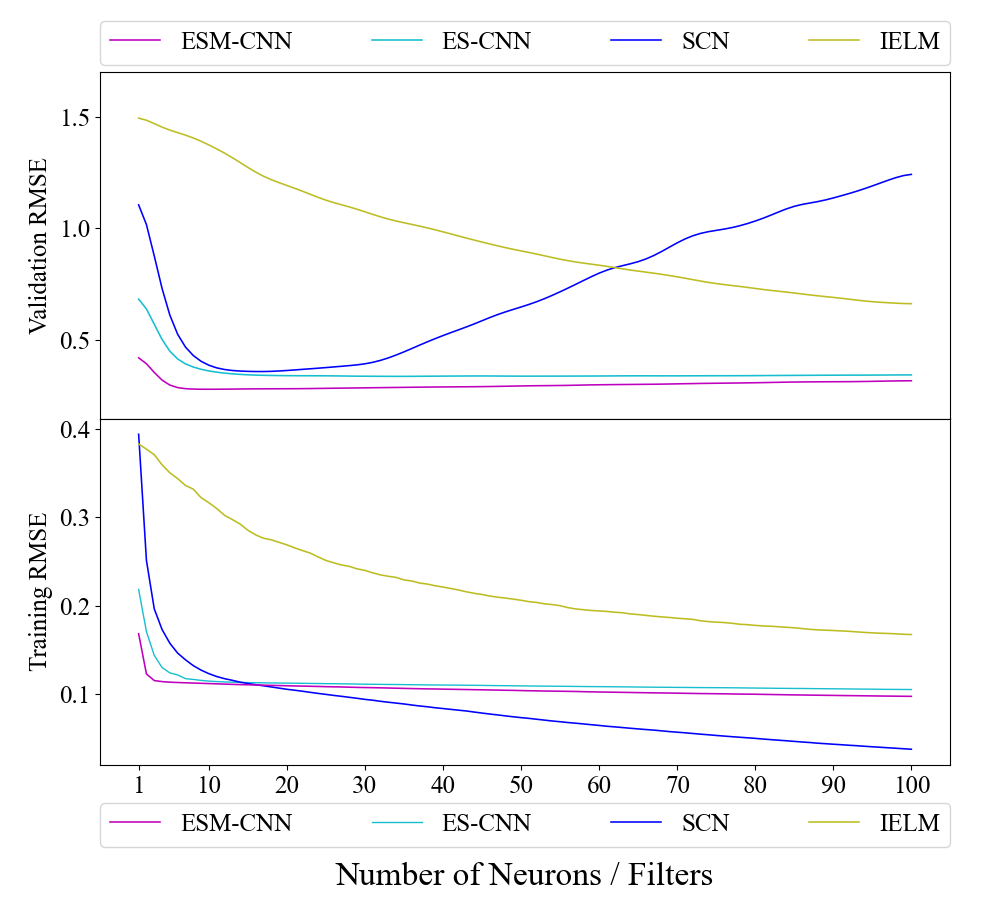
\includegraphics[width = \textwidth]{float/ch.cnn/sili_H1_revise.png}
        \subcaption{\label{fig:silih1} ILI, $H = 1$ }
    \end{minipage}
    \hspace{4em}
    \begin{minipage}[b]{0.43\textwidth}
        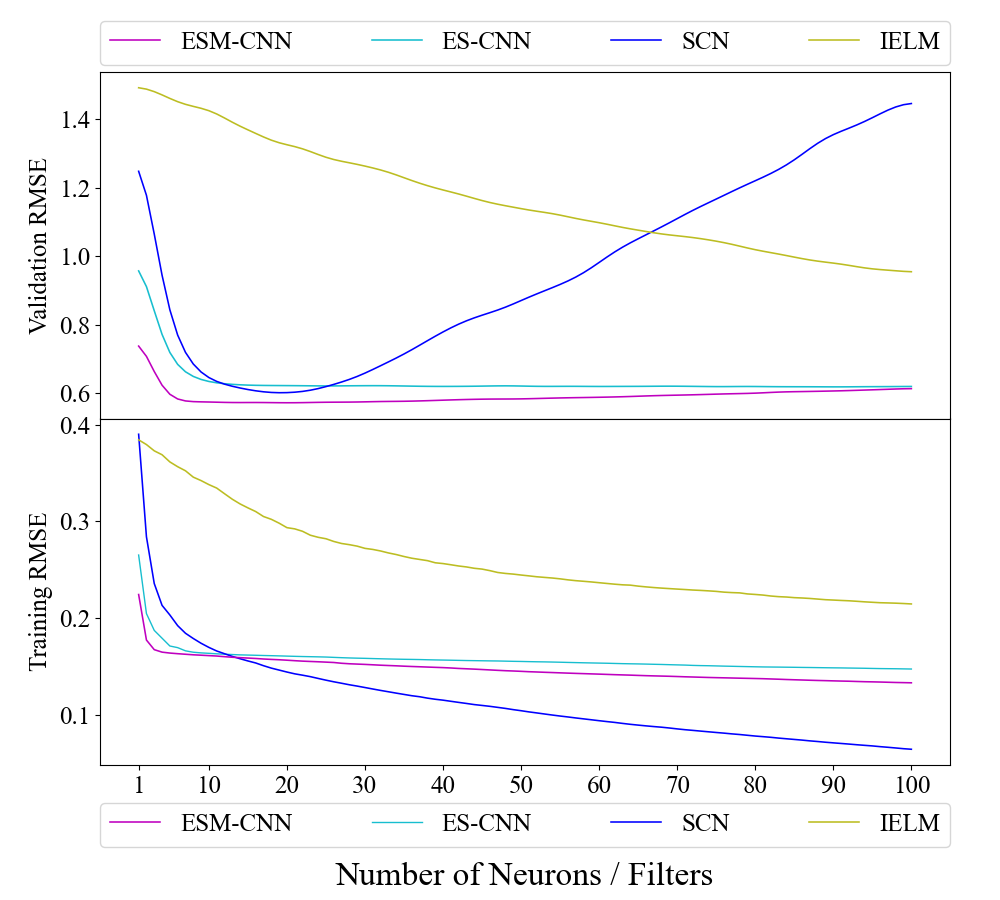
\includegraphics[width = \textwidth]{float/ch.cnn/sili_H4_revise.png}
        \subcaption{\label{fig:silih4} ILI, $H = 4$ }
    \end{minipage}
    \begin{minipage}[b]{0.43\textwidth}
        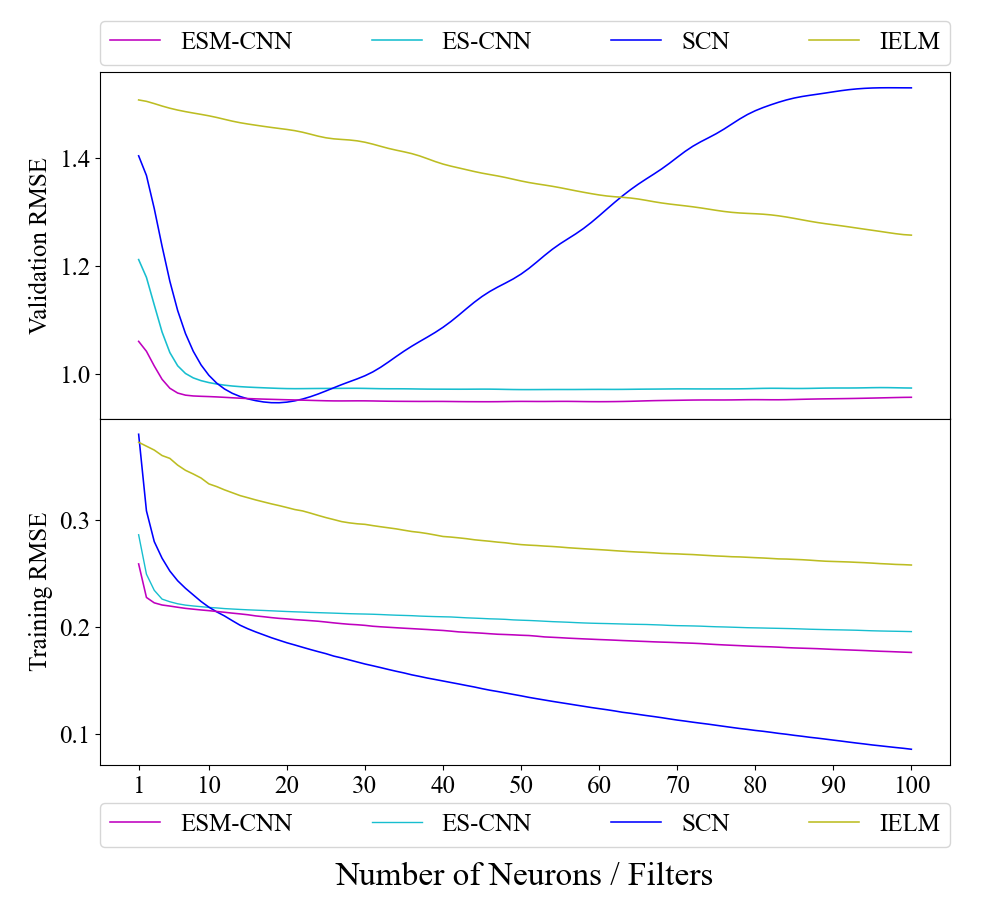
\includegraphics[width = \textwidth]{float/ch.cnn/sili_H8_revise.png}
        \subcaption{\label{fig:silih8} ILI, $H = 8$ }
    \end{minipage}

    \caption{\label{fig:converge} ILI数据集上递归增长随机映射神经网络的RMSE曲线}
\end{figure*}


\subsection{收敛效果对比与分析}
本章节对比了基于递归增长随机映射构造策略模型(即IELM、SCN、ES-CNN和ESM-CNN模型)的收敛性,以更好评价所提模型的收敛效果。
\autoref{fig:converge}绘制出了ILI数据集上随递归增长随机映射模型随隐藏层神经元或卷积核数量变化所达到的训练集与验证集RMSE曲线。基于该收敛性结果,可归纳出以下结论:

(1)同一预测模型在不同预测时长任务上的收敛情况是一致的。

(2)尽管SCN模型在不同预测任务的训练集RMSE上都能做出最快收敛,但通过验证集RMSE曲线可知,SCN模型在进行真实预测建模中出现了明显的过拟合现象,而采用误差反馈策略的IELM模型并没有出现过拟合,但表现出最慢的收敛速度。这一对比结果证明了误差反馈策略解决过拟合问题的有效性,同时也指出了误差反馈策略下MLP结构的性能局限性。

(3)基于卷积结构的ESM-CNN和ES-CNN在所有的验证集RMSE中都表现出比IELM和SCN更快且更低的收敛效果,证明了基于误差反馈随机映射构造CNN预测模型的收敛性与鲁棒性。

(4)与ES-CNN相比,ESM-CNN具备更低的训练集RMSE曲线和测试集RMSE曲线,从收敛性角度再次验证了所提卷积核选择方法的有效性与必要性。

(5)在ESM-CNN与ES-CNN的收敛过程中,预测性能的最大增益明显来自于构造过程的前10步,表现出ESM-CNN具备通过牺牲微小性能换来巨大效率提升的平衡策略,从而使得ESM-CNN具有更加广泛和高效的现实应用性。


进一步地,对于本章实验中\autoref{fig:converge}所显示的SCN与Stoc-CNN过拟合现象以及ESM-CNN与ES-CNN模型的鲁棒性特点,其解释如下:由于SCN与Stoc-CNN均采用最小二乘法全局更新输出权重的方式,使其难以克服现实复杂时间序列中的噪声数据,因此出现了过拟合的现象;与全局更新输出层权重的构造方式相反,ESM-CNN与其消融模型ES-CNN采用基于构造过程预测误差反馈局部更新输出权重的方式,随着卷积核的不断增加,一方面,既有预测误差被不断弥补,使得噪声数据的影响被不断削弱,另一方面历史加入的卷积核权重及其链接的输出权重被固定住,这些固定的权重在一定程度上充当了正则化的作用,使得新加入卷积核的输出权重$L_2$范数越来越小,并在整体上小于SCN与Stoc-CNN,从而使模型具有更高的稳定性与鲁棒性。


\subsection{建模效率对比与分析}
\begin{table*}[!t]
    \centering
    \footnotesize
    \caption{神经网络模型在AR1、BTC和ILI数据集上的单次平均建模时间(s) \label{tab:time}}
    \resizebox{\textwidth}{!}{\begin{tabular}{ccrrrrrrrrr}
        \toprule
        \multirow{2}{*}{建模方法}   & \multirow{2}{*}{模型} & \multicolumn{3}{c}{AR1} & \multicolumn{3}{c}{BTC} & \multicolumn{3}{c}{ILI}                                           \\\cmidrule(lr){3-5} \cmidrule(lr){6-8}\cmidrule(lr){9-11}
                          &                         & \multicolumn{1}{c}{1} & \multicolumn{1}{c}{3} & \multicolumn{1}{c}{6} & \multicolumn{1}{c}{1} & \multicolumn{1}{c}{3} & \multicolumn{1}{c}{6} & \multicolumn{1}{c}{1} & \multicolumn{1}{c}{4} & \multicolumn{1}{c}{8} \\ \midrule        
        
\multirow{3}{*}{梯度下降} & GS-CNN                  & 74.65                 & 76.95                 & 78.55                 & 93.70                 & 96.45                 & 99.40                 & 67.05                 & 70.25                 & 73.00                 \\
                          & DeepAR                  & 225.25                & 238.95                & 257.70                & 223.75                & 251.10                & 268.65                & 256.80                & 279.10                & 275.30                \\
                          & CLSTM                   & 150.45                & 154.80                & 160.25                & 143.00                & 141.50                & 142.25                & 167.40                & 170.80                & 175.30                \\
\specialrule{0em}{1.5pt}{1.5pt}                          
\multirow{3}{*}{随机映射}   & RVFL                    & \multicolumn{1}{c}{-} & \multicolumn{1}{c}{-} & \multicolumn{1}{c}{-} & \multicolumn{1}{c}{-}  & \multicolumn{1}{c}{-}  & \multicolumn{1}{c}{-}  & \multicolumn{1}{c}{-} & \multicolumn{1}{c}{-} & \multicolumn{1}{c}{-} \\
                          & IELM                    & 2.65                  & 2.85                  & 2.80                  & 3.40                  & 3.30                  & 3.20                  & 2.55                  & 2.55                  & 2.40                  \\
                          & SCN                     & 22.85                 & 57.40                 & 107.75                & 21.10                 & 58.00                 & 111.40                & 16.10                 & 49.60                 & 90.95                 \\
\specialrule{0em}{1.5pt}{1.5pt}                          
\multirow{2}{*}{消融方法} & Stoc-CNN                & \multicolumn{1}{c}{-} & \multicolumn{1}{c}{-} & \multicolumn{1}{c}{-} & \multicolumn{1}{c}{-}  & \multicolumn{1}{c}{-}  & \multicolumn{1}{c}{-}  & \multicolumn{1}{c}{-} & \multicolumn{1}{c}{-} & \multicolumn{1}{c}{-} \\
                          & ES-CNN                  & 6.50                  & 6.40                  & 6.50                  & 6.35                  & 6.50                  & 6.45                  & 6.45                  & 6.50                  & 6.50                  \\
\specialrule{0em}{1.5pt}{1.5pt}                          
所提方法                       & ESM-CNN                 & 9.65                  & 9.65                  & 9.70                  & 7.10                  & 7.25                  & 7.25                  & 7.15                  & 7.15                  & 7.20                  \\ \bottomrule
    \end{tabular}}
\end{table*}
此外,本章节对比了所选模型中神经网络预测模型的单次平均建模时间,以更好评价所提模型的实际建模效率。
\autoref{tab:time}展示了所选神经网络预测模型在AR1、BTC和ILI数据集上以秒为单位的单次平均建模时间。其中,因RVFL与Stoc-CNN的构造过程仅由随机初始化隐藏层权重与闭式求解输出权重两部分组成,在当前实验环境下,模型构造时间可被省略,因此用“-”进行标记。

通过对比卷积结构的训练DNN模型(即GS-CNN)与循环结构的训练DNN模型(即DeepAR和CLSTM),GS-CNN模型具有更高的建模效率,其用时约是纯循环结构模型DeepAR的三分之一,约是堆叠卷积与循环结构模型CLSTM的二分之一,验证了卷积结构的效率优势。

进一步地,结合前文的预测结果可知,ESM-CNN与ES-CNN仅需相对极少的建模时间即可达到与梯度下降训练深度学习预测模型媲美甚至更好的预测性能,同时参考\autoref{fig:converge}所示的收敛性结果可知,该建模时间仍有相当压缩空间以进一步提高建模效率,证明了误差反馈随机映射方法构造CNN模型的建模高效性。
同时,ESM-CNN与ES-CNN相比,增加的卷积核选择过程在未明显增加建模时间的情况下显著提高了预测性能,证明了ESM-CNN的建模优势。

\section{小结\label{sec:esm.conc}}


面对预测建模技术研究中卷积结构SDNN预测模型的构造与自适应优化问题,针对已有方法的诸多不足,本章提出了一种新颖的ESM-CNN预测模型,基于误差反馈随机映射建模策略和卷积参数贪心选择方法,构造出一种兼具优异建模效率与预测性能的卷积结构SDNN预测模型,并证明了其收敛性。

本章节以经典人工时间序列数据、比特币价格、流感阳性样本率、国际原油价格、股票指数等多项真实时间序列数据为预测对象,进行多个预测时长下的预测任务,基于不同预测准确度评价指标,通过预测准确度、收敛性和建模效率等多个视角的对比分析验证了所提ESM-CNN模型的性能与效率,结果表明该模型是一种兼具优秀预测性能与建模效率的卷积结构SDNN预测模型。有望基于该模型为比特币价格预测、流感阳性样本率预测、国际原油价格预测和股票指数预测等管理应用提供相比传统统计方法和传统随机映射方法更为精准的预测结果,同时可利用其远优于训练深度学习预测方法的建模效率优势,为时变或在线环境下的复杂预测管理应用问题提供可能的解决方案。